\documentclass[11pt,a4paper]{report}

% - Make more clear which version of MEDS we optimized (the one after optimization) and discuss how these optimizations could also be applied to the original one
% - 'Optimizing Cryptographic Schemes' section is relevant
% - Related Work: show landscape, elliptic curve optimization. other signature schemes. Other fiat shamir (and what is important in such schemes, such as keccak). Maybe cite other optimizations from the same NIST competition (other fiat shamir signatures maybe, if something interesting is there; LESS/uv-based/code-based/with fields). Additionally, maybe look at other techniques such as AVX2/AVX512 that are used nowadays.
% - Research goals before preliminaries. Need full chapter probably. Make sure you explain everything without too much knowledge required.
% - Start every chapter with a small summary (but no forward references)
% - Definitely do include complexity for matrix systemization
% - If you don't include a complexity, give an operation count
% - All referneces to 'solve' need to be altered a bit. Give pseudocode/algorithm for 'solve' in the appendix and explain what it does.
% - In every figure and table, give references in the caption to all the sources.
% - Definitely include comparison to other schemes; Dilithium(?), Falcon(?), Sphinx(?), traditional ECC(?), SELF REPORTED!!

\usepackage{algorithm}
\usepackage[noend]{algpseudocode}
\usepackage{algpseudocode}
\usepackage{amsmath}
\usepackage{amssymb}
\usepackage{amsthm}
\usepackage[english]{babel}
\usepackage{booktabs}
\usepackage{dsfont}
\usepackage{enumitem}
\usepackage{etoolbox}
\usepackage[a4paper]{geometry}
\usepackage{graphics}
\usepackage{graphicx}
\usepackage{hyperref}
\usepackage[utf8]{inputenc}
\usepackage{listings}
\usepackage{natbib}
\usepackage{parskip}
\usepackage{pgf-pie}
\usepackage{tabularx}
\usepackage{todonotes}
\usepackage{url}
\usepackage{xcolor}
\usepackage{xurl}

\interfootnotelinepenalty=10000

% Define nice pie chart colors
\definecolor{pie1}{HTML}{03045e}
\definecolor{pie2}{HTML}{023e8a}
\definecolor{pie3}{HTML}{0077b6}
\definecolor{pie4}{HTML}{0096c7}
\definecolor{pie5}{HTML}{00b4d8}
\definecolor{pie6}{HTML}{48cae4}
\definecolor{pie7}{HTML}{90e0ef}
\definecolor{pie8}{HTML}{ade8f4}
\definecolor{pie9}{HTML}{caf0f8}

\setlength{\marginparwidth}{2cm}
\hypersetup{
    colorlinks,
    citecolor=black,
    filecolor=black,
    linkcolor=black,
    urlcolor=black
}

\newtheorem{theorem}{Theorem}
\theoremstyle{definition}
\newtheorem{definition}{Definition}[section]
\AtBeginEnvironment{definition}{\vspace{1em}}

\lstdefinestyle{CStyle}{
  language=C,
  commentstyle=\color{green!60!blue},
  keywordstyle=\color{blue},
  numberstyle=\tiny\color{black!80},
  stringstyle=\color{green},
  basicstyle=\footnotesize\ttfamily,
  breakatwhitespace=false,         
  breaklines=true,                 
  captionpos=b,                    
  keepspaces=true,                 
  numbers=left,                    
  numbersep=5pt,                  
  showspaces=false,                
  showstringspaces=false,
  showtabs=false,                  
  tabsize=2,
  morekeywords={uint64_t, pmod_mat_entry, uint16x4_t, uint32x4_t, uint64x2_t, vmull_u32, vget_low_u32, vmull_high_u32, vuzp2q_u32, vshrq_n_u32, vmlsq_u32, vmovn_u32, pmod_mat_t, pmod_mat_vec_t, pmod_mat_vec_w_t, ZERO_VEC_W, MUL_ACC_VEC, FREEZE_REDUCE_VEC}
}


\lstdefinestyle{ASMStyle}{
  language=C,
  commentstyle=\color{green!60!blue},
  keywordstyle=\color{blue},
  numberstyle=\tiny\color{black!80},
  stringstyle=\color{green},
  basicstyle=\footnotesize\ttfamily,
  breakatwhitespace=false,         
  breaklines=true,                 
  captionpos=b,                    
  keepspaces=true,                 
  numbers=left,                    
  numbersep=5pt,                  
  showspaces=false,                
  showstringspaces=false,
  showtabs=false,                  
  tabsize=2,
  morekeywords={umull, umull2, uzp2, ushr, mls, xtn}
}

% Set the line spacing between paragraphs
% \setlength{\parskip}{1em}
% Remove paragraph indentation
% \setlength{\parindent}{0pt}

% URL LINE BREAKS
\expandafter\def\expandafter\UrlBreaks\expandafter{\UrlBreaks% save the current one
  \do\a\do\b\do\c\do\d\do\e\do\f\do\g\do\h\do\i\do\j%
  \do\k\do\l\do\m\do\n\do\o\do\p\do\q\do\r\do\s\do\t%
  \do\u\do\v\do\w\do\x\do\y\do\z\do\A\do\B\do\C\do\D%
  \do\E\do\F\do\G\do\H\do\I\do\J\do\K\do\L\do\M\do\N%
  \do\O\do\P\do\Q\do\R\do\S\do\T\do\U\do\V\do\W\do\X%
  \do\Y\do\Z\do\*\do\-\do\~\do\'\do\"\do\-}%

\makeatletter %otherwise geometry resets everything
\Gm@restore@org
\makeatother

\setlength{\itemsep}{0cm}
\setlength{\voffset}{0cm}
\setlength{\headheight}{0cm}
\setlength{\topmargin}{0cm}

\graphicspath{{imgs/}}

\begin{document}
\begin{titlepage}
  \begin{center}
    \textsc{\LARGE Master Thesis\\Computing Science}\\[1.5cm]
    
\includegraphics[height=100pt]{logo}

    \vspace{0.4cm}
    \textsc{\Large Radboud University}\\[1cm]
    \hrule
    \vspace{0.4cm}
    \textbf{\huge Optimizing the MEDS implementation for ARMv8}\\[0.4cm]
    \vspace{0.2cm}
    \hrule
    \vspace{2cm}
    \begin{minipage}[t]{0.45\textwidth}
      \begin{flushleft} \large
        \textit{Author:}\\
        Lars Jeurissen\\
        s1022856\\
        \texttt{\href{mailto:lars.jeurissen@ru.nl}{lars.jeurissen@ru.nl}}
      \end{flushleft}
    \end{minipage}
    \begin{minipage}[t]{0.45\textwidth}
      \begin{flushright} \large
        \textit{First supervisor/assessor:}\\
        prof. dr. Peter Schwabe\\
        \texttt{\href{mailto:p.schwabe@cs.ru.nl}{p.schwabe@cs.ru.nl}}\\[1.3cm]
        \textit{Second supervisor:}\\
        dr. Simona Samardjiska\\
        \texttt{\href{mailto:simonas@cs.ru.nl}{simonas@cs.ru.nl}}
      \end{flushright}
    \end{minipage}
    \vfill
    {\large \today}
  \end{center}
\end{titlepage}

\renewcommand{\abstractname}{Acknowledgements}
\begin{abstract}
Thank you.
\end{abstract}

\renewcommand{\abstractname}{Abstract}
\begin{abstract}
Abstract.

%The abstract of your thesis is a brief description of the research hypothesis,
%scientific context, motivation, and results.
%The preferred size of an abstract is one paragraph or one page of text.
\end{abstract}

\tableofcontents
\newpage

\chapter{Introduction}
\label{ch:introduction}
As the research on quantum computers progresses, we are getting increasingly closer to the point where quantum computers will be able to utilize algorithms such as Shor's algorithm \cite{shor1994algorithms} and Grover's algorithm \cite{grover1996fast} to break a lot of symmetric and asymmetric cryptographic schemes. As the majority of the internet's security relies on these cryptographic schemes, the consequences of this are severe. Without proper measurements, quantum computers will cause the absolute collapse of the present public key algorithms that are considered secure \cite{mavroeidis2018impact}, wich would have devestating consequences for the security of the internet.

The solution to this problem lies in the development of cryptographic schemes that are secure against quantum computers. Such algorithms have been around for a long time, but this area of research has experienced a boost in attention ever since the National Institute of Standards and Technology (NIST) started the post-quantum cryptography (PQC) standardization process in 2017 \cite{nist2017pqc}. The goal of this process is to standardize cryptographic schemes that are secure against quantum computers.

In 2022, NIST announced the set of selected PQC algorithms. Unfortunately, this set did not include any algorithms for digital signatures. To address this, NIST announced a second competition in the PQC standardization process, which aims to find a set of secure digital signature schemes. One of the candidates in this competition is Matrix Equivalence Digital Signature (MEDS) \cite{chou2023take}. MEDS is a code-based digital signature scheme based on the notion of Matrix Code Equivalence.

Although the MEDS scheme is actively being optimized in terms of key and signature sizes, the performance of the scheme is still lacking. The reported signature verification times are in the order of hundreds of milliseconds, sometimes even seconds.

In this thesis, we aim to optimize the speed of the MEDS implementation. We will look at the general performance of MEDS, but we will mostly focus on the ARMv8 architecture. This architecture is used in a wide range of devices, including many mobile devices and tablets, Internet of Things (IoT) devices, and Apple M1/M2 chips. By optimizing the MEDS implementation for ARMv8, we aim to improve the MEDS performance for these devices, as well as obtain a better understanding of the performance of MEDS.

We investigate the following research questions in this thesis (see also Chapter \ref{ch:researchobjectives}):
\begin{itemize}
  \item What are the bottlenecks in the MEDS implementation?
  \item How can we improve the general performance of the MEDS implementation?
  \item How can we optimize the MEDS implementation for ARMv8?
  \item How does the optimized MEDS implementation compare to (optimized) implementations of other digital signature schemes?
\end{itemize}

In Chapter \ref{ch:preliminaries}, we will provide the necessary background information on the functioning of MEDS and the specific details of the ARMv8 architecture. In Chapter \ref{ch:researchobjectives}, we will discuss the research objectives of this thesis. In Chapter \ref{ch:profiling}, we discuss the profiling techniques that we use to obtain an understanding of the performance of MEDS. In this Chapter, we will also present the profiling results of the MEDS implementation. Following that, in Chapter \ref{ch:methodology}, we will discuss the optimization techniques that we use to optimize the MEDS implementation. In Chapter \ref{ch:results}, we will present the benchmarking results of the non-optimized and optimized MEDS versions and compare these results to other digital signature schemes. Finally, in Chapter \ref{ch:futurework}, we will discuss the future work that can be done in this area. We will conclude the thesis in Chapter \ref{ch:conclusion}, where we will reflect on the research questions and the results that we have obtained.

\chapter{Preliminaries}
\label{ch:preliminaries}

\section{Notations}
\label{sec:notations}
In the MEDS scheme and in this thesis, we use the following notations and definitions:
\begin{itemize}
  \item $\mathbb{F}_q$: The finite field of size $q$.
  \item $\mathbb{F}_q^{m \times n}$: The set of matrices of size $m \times n$ ($m$ rows and $n$ columns) over $\mathbb{F}_q$, meaning that each element of the matrix is an element of $\mathbb{F}_q$.
  \item $\textbf{A} \in \mathbb{F}_q^{m \times n}$: A matrix $\textbf{A}$ of size $m \times n$ over $\mathbb{F}_q$.
  \item $\textbf{A}[i][j]$: The element in the $i$-th row and $j$-th column of matrix $\textbf{A}$.
  \item $\textbf{A}^T$: The transpose of matrix $\textbf{A}$.
  \item $\textbf{A}^{-1}$: The inverse of matrix $\textbf{A}$.
  \item $\textbf{A} \times \textbf{B}$ or simply $\textbf{AB}$: The matrix product of $\textbf{A}$ and $\textbf{B}$.
  \item $\textbf{A} + \textbf{B}$: The matrix sum of $\textbf{A}$ and $\textbf{B}$.
  \item $\textbf{A} \otimes \textbf{B}$: The Kronecker product of $\textbf{A}$ and $\textbf{B}$.
  \item $\pi_{\textbf{A}, \textbf{B}}(\textbf{G})$: Simplified notation for the operation $\textbf{G}(\textbf{A}^T \otimes \textbf{B})$.
\end{itemize}

\section{Matrix Equivalence Digital Signature (MEDS)}
\label{sec:meds}
Matrix Equivalence Digital Signature (MEDS) \cite{chou2023take} is a code-based digital signature scheme and the candidate in the NIST PQC competition that we aim to optimize in this thesis. A series of optimizations for the key and signature sizes of MEDS have already been proposed by the authors of the scheme in \cite{chou2024reducing}, together with a new reference implementation that implements these optimizations. In this paper, we will focus our efforts on optimizing this new reference implementation.

\subsection{Signature Schemes}
\label{sec:signatureschemes}
A digital signature scheme is a cryptographic scheme with the purpose of verifying the authenticity of a message. The scheme allows a party to sign a piece of data such as a message or a document, after which any party can verify the signature and thereby the authenticity of the data.

A digital signature scheme consists of three algorithms:
\begin{itemize}
  \item \textbf{Key generation}: This algorithm generates 2 keys, a private key and a public key. The private key is used to sign the data, and the public key is used to verify the signature.
  \item \textbf{Signature generation}: Given a message and the private (and sometimes public) key, this algorithm generates a signature for the message.
  \item \textbf{Signature verification}: Given a message, a signature, and the public key, this algorithm verifies the signature.
\end{itemize}
The formal definition of a digital signature scheme is given in Definition \ref{def:signaturescheme}.

\begin{definition}[Signature Scheme, following \cite{goldwasser2008lecture}]~\\
  \label{def:signaturescheme}
  A digital signature scheme is a tuple of algorithms $(\text{G}, \text{S}, \text{V})$, where:
  \begin{itemize}
    \item $\text{G}(1^n)$ generates a key pair $(pk, sk)$, where $pk$ is the public key and $sk$ is the private key. The parameter $n$ represents the security parameter which determines the security level of the scheme.
    \item $\text{S}(sk, m)$ generates a tag $T$ which represents the signature of the message $m$ using the private key $sk$.
    \item $\text{V}(pk, m, T)$ outputs 1 if the tag $T$ is a valid signature of the message $m$ using the public key $pk$, and 0 otherwise.
  \end{itemize}
  Such that, given $(pk, sk) \leftarrow \text{G}(1^n)$:
  \[
    \text{V}(pk, m, \text{S}(sk, m)) = 1
  \]
  for all $m$ (with a negligible probability of error).
\end{definition}

\subsection{How MEDS Works}
\label{sec:medsworks}
Most PQC schemes are based on mathematical concepts such as linear codes, isogenies, lattices and multivariate equations. These concepts have associated decisional and computational problems that are believed to be hard to solve for both classical and quantum computers. MEDS is based on the notion of Matrix Code Equivalence, which is closely related to the notion of Code Equivalence that is used in LESS \cite{biasse2020less}, a similar scheme in the NIST PQC Signature competition.

\subsubsection{The Matrix Code Equivalence (MCE) Problem}
MEDS bases its security on the hardness of the Matrix Code Equivalence (MCE) problem. The computational form of this problem is shown in Definition \ref{def:mceproblem}.

\begin{definition}[Matrix Code Equivalence Problem, following \cite{chou2023meds}]~\\
  \label{def:mceproblem}
  Given two rank metric codes $\mathcal{C}, \mathcal{D}$ of size $[m \times n, k]$,\\
  find an isometry $\phi$ on $\mathbb{F}_q^{m \times n}$ such that $\mathcal{C} = \phi(\mathcal{D})$.\\
  An isometry $\phi$ is an $\mathbb{F}_q$-linear map that preserves the rank of matrices. 
\end{definition}

For more information, we refer the reader to \cite{reijnders2024hardness}, where the problem is explained in more detail and its hardness is studied.

\subsubsection{Sigma Protocol}
\label{sec:sigmaprotocol}
The MCE problem is used in MEDS to construct a 3-pass Sigma protocol \cite{damgaard2002sigma}. A Sigma protocol is a protocol between a prover and a verifier where the prover convinces the verifier that it knows a piece of information without revealing the information itself. In the case of MEDS, the prover convinces the verifier that it knows a certain isometry $\phi$ that satisfies the MCE problem. The Sigma protocol for the optimized version of MEDS is provided in \cite[Section 4.2]{chou2024reducing}.

\subsubsection{Fiat-Shamir Transform}
\label{sec:fiatshamir}
To convert a Sigma protocol into a usable digital signature scheme, the Fiat-Shamir transform \cite{fiat1986prove} is used. The initial Sigma protocol is interactive, meaning that the prover and verifier exchange messages, which is not suitable for a digital signature. The Fiat-Shamir transform converts the Sigma protocol such that the prover can show knowledge of the isometry while only sending a single message to the verifier, making it non-interactive. This is achieved by creating the challenge based on a collision-resistant hash of the message to be signed and the commitments for each round.

When working with the Fiat-Shamir transform, various techniques and optimizations can be used to increase the security or lower the size of the public key and the signature. The following techniques are considered in the MEDS scheme:
\begin{itemize}
  \item \textbf{Multiple Challenges}:\\
  An attacker can impersonate an honest prover with $\frac{1}{2}$ probability. To prevent this, the scheme can use $t$ challenges, reducing the probability of impersonation to $\frac{1}{2^t}$.
  \item \textbf{Multiple Public Keys}:\\
  As mentioned before, an attacker can impersonate an honest prover with $\frac{1}{2}$ probability. To reduce this probability, the scheme can use multiple public keys, each of which is used to compute a different isometry. This increases the challenge space from $2$ to $s$, reducing the probability of impersonation to $\frac{1}{s}$ ($s$ is the number of public keys used in the scheme).
  \item \textbf{Fixed-Weight Challenge Strings}:\\
  If a challenge is 0, the response consists of matrices that are generated uniformly at random. In this case, it is sufficient to set the response to the seed that was used to generate the matrices, greatly reducing the size of the signature. By fixing a certain number $w$ of challenges to 0, the average size of a response can be reduced. This technique has a slightly negative impact on the security of the scheme, but this can be compensated by increasing the number of challenges.
  \item \textbf{Seed Tree}:\\
  If a scheme requires sending multiple seeds for the generation of matrices (or other objects), a seed tree can be used to reduce the size of the public key and the signature. This is a structure that allows the prover to transmit a smaller amount of bits than the size of the seeds, at the cost of an increased computational complexity.
\end{itemize}

By selecting $t$, $s$ and $w$ carefully and combining them with other parameters of the scheme, the security of the scheme can be increased to the desired level. Multiple combinations of parameters are used in MEDS to achieve various security levels \cite{chou2023meds}. The selection of these parameters has a big influence on the size of the public key and the signature, as well as the computational performance of the scheme.

\subsection{Parameter Sets}
\label{sec:parametersets}
The security of MEDS depends on the choice of a set of parameters. The parameters that are used in the MEDS scheme are the following:
\begin{itemize}
  \item $q$: The size of the finite field $\mathbb{F}_q$ over which all computations are done.
  \item $n$: The width and height of the private matrices $A_i \in \mathbb{F}_q^{n \times n}$ that are used to generate the key pair.
  \item $m$: The width and height of the private matrices $B_i \in \mathbb{F}_q^{m \times m}$ that are used to generate the key pair.
  \item $k$: The width and height of the private matrices $T_i \in \mathbb{F}_q^{k \times k}$ that are used to generate the key pair.
  \item $s$: The number of different public keys that are used in the scheme.
  \item $t$: The number of challenges that are used in the Fiat-Shamir transform.
  \item $w$: The number of challenges in the Fiat-Shamir transform that are fixed to be 0.
\end{itemize}

The team behind MEDS has proposed three parameter sets for the new optimized version of the scheme. These parameter sets are optimized for the three different security levels that are required in the NIST PQC competition. The parameter sets are shown in Table \ref{tab:medsparametersets}. The security level for each parameter set is shown in Table \ref{tab:medssecuritylevels}.

\begin{table}
  \centering
  \begin{tabular}{lccccccccc}
    \toprule
    \textbf{Parameter Set} & \textbf{$q$} & \textbf{$n$} & \textbf{$m$} & \textbf{$k$} & \textbf{$s$} & \textbf{$t$} & \textbf{$w$} & \textbf{pk} & \textbf{sig} \\
    \midrule
    MEDS-21595 & 4093 & 26 & 25 & 25 & 2 & 144 & 48 & 21595 & 5200 \\
    MEDS-55520 & 4093 & 35 & 34 & 34 & 2 & 208 & 75 & 55520 & 10906 \\
    MEDS-122000 & 4093 & 45 & 44 & 44 & 2 & 272 & 103 & 122000 & 19068 \\
    \bottomrule
  \end{tabular}
  \caption{MEDS Parameter Sets. \textbf{pk} and \textbf{sig} represent the size in bytes of the public key and the signature, respectively.}
  \label{tab:medsparametersets}
\end{table}

\begin{table}
  \centering
  \begin{tabular}{lcc}
    \toprule
    \textbf{Parameter Set} & \textbf{NIST Category} & \textbf{FS} \\
    \midrule
    MEDS-21595 & Level 1 & -128.406 \\
    MEDS-55520 & Level 3 & -192.058 \\
    MEDS-122000 & Level 5 & -256.005 \\
    \bottomrule
  \end{tabular}
  \caption{MEDS Security Levels. \textbf{FS} denotes the claimed security of a MEDS parameter set in bits.}
  \label{tab:medssecuritylevels}
\end{table}

We can see that all parameter sets use the same finite field size $q = 4093$. The dimensions of the matrices that are used increase with each security level, as well as the number of challenges $t$ (and the number of fixed challenges $w$). The number of public keys $s$ is always set to 2, meaning the scheme does not use the multiple public keys technique, which would have greatly increased the size of the public key and the signature. Note that this differs from the original MEDS scheme, which used multiple public keys \cite{chou2023meds}.

% A section that references the 3 meds algorithms of which the pseudocode is shown in the appendix
\subsection{MEDS Algorithms}
\label{sec:medsalgorithms}
In this section, we will give an algorithmic overview of the three algorithms of MEDS: key generation, signature generation, and signature verification. The complete and detailed pseudocode of these algorithms is shown in Appendix \ref{app:medsalgs}.

\subsubsection{Key Generation}
% This section will contain an algorithm that represents key generation. It is not the completely detailed variant (which is shown in the appendix), but a more high-level overview of the algorithm.
A simplified overview version of the MEDS key generation algorithm is shown in Algorithm \ref{alg:medskeygenoverview}. The full and detailed key generation algorithm for MEDS is shown in Algorithm \ref{alg:medskeygen} (Appendix \ref{app:medsalgs}).

\begin{algorithm}
  \caption{MEDS Key Generation (Overview)}
  \label{alg:medskeygenoverview}
  \begin{algorithmic}[1]
    \State \textbf{Input:} -
    \State \textbf{Output:} Public key \textbf{pk}, private key \textbf{sk}
    \State Generate random matrix $\textbf{G}_0 \in \mathbb{F}_q^{k \times mn}$
    \For{$i = 1$ to $s$}
      \State Generate random invertible matrix $\textbf{T}_i \in \mathbb{F}_q^{k \times k}$
      \State Compute $\textbf{G}'_{0} \in \mathbb{F}_q^{k \times mn} = \textbf{T}_i \times \textbf{G}_0$
      \State Solve $\textbf{G}'_{0}$ to obtain $\textbf{A}_i \in \mathbb{F}_q^{m \times m}$ and $\textbf{B}_i \in \mathbb{F}_q^{n \times n}$
      \State Compute $\textbf{G}_i \in \mathbb{F}_q^{k \times mn} = \pi_{\textbf{A}_i, \textbf{B}_i}(\textbf{G}_0)$
      \State Convert $\textbf{G}_i$ to systematic form
    \EndFor
    \State \Return pk $= \textbf{G}_0, \textbf{G}_i$, sk $= \textbf{G}_0, \textbf{A}_i, \textbf{B}_i, \textbf{T}_i$ (for $i = 1$ to $s$)
  \end{algorithmic}
\end{algorithm}

\subsubsection{Signature Generation}
A simplified overview version of the MEDS signature algorithm is shown in Algorithm \ref{alg:medssignoverview}. The full and detailed signature generation algorithm for MEDS is shown in Algorithm \ref{alg:medssign} (Appendix \ref{app:medsalgs}).

\begin{algorithm}
  \caption{MEDS Signature Generation (Overview)}
  \label{alg:medssignoverview}
  \begin{algorithmic}[1]
    \State \textbf{Input:} Private key \textbf{sk}, message $m$
    \State \textbf{Output:} Signature $s$ (contains the tag)
    \State Parse $\textbf{G}_0$ and $\textbf{T}_i$ from \textbf{sk} for $i = 1$ to $s$
    \For{$i = 0$ to $t$}
      \State Generate random matrix $\tilde{\textbf{M}}_i \in \mathbb{F}_q^{2 \times k}$
      \State Compute $\textbf{C} \in \mathbb{F}_q^{2 \times mn} = \tilde{\textbf{M}}_i \times \textbf{G}_0$
      \State Solve $\textbf{C}$ to obtain $\textbf{A} \in \mathbb{F}_q^{m \times m}$ and $\textbf{B} \in \mathbb{F}_q^{n \times n}$
      \State Compute $\tilde{\textbf{G}}_i \in \mathbb{F}_q^{2 \times mn} = \pi_{\textbf{A}, \textbf{B}}(\textbf{G}_0)$
      \State Convert $\tilde{\textbf{G}}_i$ to systematic form
    \EndFor
    \State Hash $m$ and $\tilde{\textbf{G}}_i$ for $i = 0$ to $t$ to obtain $d$
    \State Parse a set of hashes $h_0, \ldots, h_{t-1}$ from $d$
    \For{$i = 0$ to $t$}
      \If{$h_i > 0$}
        \State Compute $\kappa_i \in \mathbb{F}_q^{2 \times k} = \tilde{\textbf{M}}_i \times \textbf{T}^{-1}_{h_i}$
      \EndIf
    \EndFor
    \State \Return Signature $s = \kappa_0, \ldots, \kappa_{t-1}, h_0, \ldots, h_{t-1}, m$
  \end{algorithmic}
\end{algorithm}

\subsubsection{Signature Verification}
A simplified overview version of the MEDS signature verification algorithm is shown in Algorithm \ref{alg:medsverifyoverview}. The full and detailed signature verification algorithm for MEDS is shown in Algorithm \ref{alg:medsverify} (Appendix \ref{app:medsalgs}).

\begin{algorithm}
  \caption{MEDS Signature Verification (Overview)}
  \label{alg:medsverifyoverview}
  \begin{algorithmic}[1]
    \State \textbf{Input:} Public key \textbf{pk}, signature $s$
    \State \textbf{Output:} 1 if the signature is valid, 0 otherwise
    \State Parse $\textbf{G}_0$ and $\textbf{G}_i$ from \textbf{pk} for $i = 0$ to $s$
    \State Parse $\kappa_i$, $h_i$, $d$ and $m$ from $s$ for $i = 0$ to $t$
    \For{$i = 0$ to $t$}
      \If{$h_i > 0$}
        \State Compute $\textbf{G}'_{0} = \kappa_i \times \textbf{G}_{h_i}$
        \State Solve $\textbf{G}'_{0}$ to obtain $\textbf{A} \in \mathbb{F}_q^{m \times m}$ and $\textbf{B} \in \mathbb{F}_q^{n \times n}$
      \Else
        \State Re-generate matrix $\tilde{\textbf{M}}_i \in \mathbb{F}_q^{2 \times k}$ as in Algorithm \ref{alg:medssignoverview}
        \State Compute $\textbf{C} \in \mathbb{F}_q^{2 \times mn} = \tilde{\textbf{M}}_i \times \textbf{G}_0$
        \State Solve $\textbf{C}$ to obtain $\textbf{A} \in \mathbb{F}_q^{m \times m}$ and $\textbf{B} \in \mathbb{F}_q^{n \times n}$
      \EndIf
      \State Compute $\hat{\textbf{G}}_i \in \mathbb{F}_q^{2 \times mn} = \pi_{\textbf{A}, \textbf{B}}(\textbf{G}_0)$
      \State Convert $\hat{\textbf{G}}_i$ to systematic form
    \EndFor
    \State Hash $m$ and $\hat{\textbf{G}}_i$ for $i = 0$ to $t$ to obtain $d'$
    \State \Return 1 if $d = d'$, 0 otherwise
  \end{algorithmic}
\end{algorithm}

\subsection{Known Attacks}
\todo[inline]{Question to Peter and Simona: Should I add a section containing a list of the best known attack(s) on MEDS (or the underlying problem)? Alternatively, I can reference the MEDS paper for this information.}

\section{ARMv8 and NEON}
\label{sec:armv8}
\todo[inline]{Cite NEON reference manual and intrinsics page.}
In this thesis, we will focus on optimizing the MEDS implementation for the ARMv8 architecture. To this end, we will use a Raspberry Pi 4 Model B, which has a 64-bit quad-core ARM Cortex-A72 CPU. We will be testing and comparing the performance of the MEDS implementation on this device.

\subsection{ARMv8 Architecture}
ARMv8 is the architecture that is used in the ARM Cortex-A72 and a lot of other processors. The default instruction set for ARMv8 is AArch64, a 64-bit instruction set that has more registers and higher performance than the 32-bit AArch32 instruction set.

\subsection{Vectorization and SIMD}
Single Instruction, Multiple Data (SIMD) is a type of instruction that operates on multiple pieces of data in parallel. Using this technique, it is possible to execute a single operation (such as an addition or multiplication) on multiple numbers in a time that is similar to the conventional operation on a single number. This can greatly improve the performance of algorithms that lend themselves to parallelization.

In ARM, the SIMD instruction set is called NEON or Advanced SIMD (both terms refer to the same thing). NEON is a 128-bit SIMD architecture extension that is required in all standard ARMv8 implementations \cite{ARMv8A-ProgrammersGuide}. The NEON unit consists of 32 128-bit registers, each of which can be used to store 16 8-bit integers, 8 16-bit integers, 4 32-bit integers, or 2 64-bit integers. The NEON instruction set includes a wide range of instructions that can be used to perform operations on these registers.

\todo[inline]{Maybe extend this section to give a more detailed explanation of NEON, such as provide lane distribution options and some operation examples, together with graphics.}

\subsection{Assembly Instructions and Latency}
\todo[inline]{For NEON; add pipeline information and latency for used assembly instructions. Include a reference to the document that provides these values.}

\subsection{Optimizing Cryptographic Schemes}
\todo[inline]{Question to Peter and Simona: I'm not completely sure if this subsection is necessary, but it would be a nice place to explain constant-time programming, timing attacks, and cache poisoning attacks. Is it a good idea to include this information?}

\section{Related Work}
\todo[inline]{Give more related work. This section will be expanded to include more related work (and references) and explanations for each item.}
\begin{itemize}
  \item The two GitHub repositories for the low-level and high-level optimizations of tradidional MEDS.
  \item Other post-quantum (signature) schemes that have been optimized for ARMv8.
  \item KECCAK (and SHAKE256).
  \item The extended KECCAK code package.
  \item The KECCAK optimization for ARMv8.
\end{itemize}

\chapter{Research Objectives}
\label{ch:researchobjectives}
\todo[inline]{Question to Peter and Simona: I'm not really certain about the necesity of this chapter. I could also include this information in the Introduction chapter. In this chapter, I would discuss the research objectives and the reason for optimizing MEDS for ARMv8.}
\todo[inline]{Explain MEDS speedup goals}
\todo[inline]{Explain SIMD speedup}
\todo[inline]{Explain ARM speedup goals (IoT, mobile, etc.)}

\chapter{Profiling}
\label{ch:profiling}
\section{Profiling Techniques}
In order to obtain a better understanding of the performance of (specific functions of) MEDS, we need to profile the implementation. Profiling is the process of measuring the space or time complexity of a program or a specific function. The goal of profiling is to identify the bottlenecks in the speed or memory usage of a program, these are the parts of the program that take the most time or memory. Usually, we hope that a small part of the program is responsible for a large part of the time or memory usage, and that this part can be optimized to improve the overall performance.

Typically, profiling is done by running the program with a profiler, which is a tool that measures the space or time that is used by the program or a specific functions. There exist a wide variety of profilers for C, such as GProf \cite{graham1982gprof}, Valgrind \cite{nethercote2007valgrind}, and Linux-Perf \cite{de2010new}. In our case, the most accurate way to measure the performance is to measure the number of cycles that are used by the program or a specific function, which can be done with Linux-Perf.

\subsection{Cycle Counting}
Cycle counting is a technique that is used to measure the number of CPU cycles that it takes to execute a certain program or function. This is usually done by accessing the performance monitoring unit (PMU) of the CPU, which is a CPU component that measures the performance of the processor. Typically, these PMUs contain a register that can be read to obtain the number of cycles executed since a certain point in time. On Linux, it is very easy to access this data using the Linux-Perf tool \cite{de2010new}, which can be used to measure the number of instructions executed, number of cache misses, etc.

\subsubsection{Advantages}
The advantages of profiling the code using a cycle counter are:
\begin{itemize}
  \item \textbf{Exact}: Measuring the cycle counter results in the most exact measurement of time. For comparison, using a technique that measures the current time in (nano)seconds is less accurate, because the CPU is capable of executing multiple cycles in a single nanosecond.
  \item \textbf{Low Overhead}: Measuring the cycle counter has a very low additional performance overhead to the program, as it usually consists of reading a single register.
  \item \textbf{Precise}: By annotating the code with our own cycle counter, we can measure the performance of specific functions or even specific lines of code.
\end{itemize}

\subsubsection{Disadvantages}
The disadvantages of profiling the code using a cycle counter are:
\begin{itemize}
  \item \textbf{Interference}: The program to be measured shares the CPU (core) with other programs, which can interfere with measurements. If another program is switched in by the operating system, the cycle counter will also count the cycles that were used by this program. Although this usually doesn't have a big impact on profiling results, this can be problematic for obtaining accurate benchmarks.
  \item \textbf{Architecture}: The way in which the cycle counter is accessed is different for each architecture. However, since we use the perf tool, this is abstracted away for us.
\end{itemize}

\subsubsection{Problem Mitigation}
There are a few problems with cycle counting that we need to mitigate. First of all, there are a few features on modern CPUs that will cause this technique to produce inaccurate results. These features include frequency scaling (based on the current workload, a CPU can change its clock frequency to save power) and hyperthreading (multiple threads share the same CPU core). It is essential to disable these features to obtain accurate results.

Another problem is the problem of program interference (see above). Unfortunately, this is a problem that is hard to prevent completely, but we can work around it. By running the program multiple times and taking the median of the results, we can reduce the impact of interference on the results. This is a common technique in benchmarking.

\section{MEDS Profiling Results}
\label{sec:medsprofilingresults}

\subsection{Measurement Setup}
We added cycle count measurements to all MEDS functions that we anticipate will require a significant amount of time. We ran our profiling tests on a Raspberry Pi 4 Model B with a 64-bit quad-core ARM Cortex-A72 CPU clocked at 1.5 GHz. We decided to profile the code for the MEDS-55520 parameter set, which is in the middle of the three parameter sets in terms of security level. The results will be representative for the other parameter sets as well. We executed measurements for the three algorithms of a digital signature scheme: key generation, signing, and verification. The results are shown in Tables \ref{tab:medskeygenfunctions} (key generation), \ref{tab:medssigningfunctions} (signing), and \ref{tab:medsverificationfunctions} (verification). For each algorithm, we list the functions or code sections that take up more than 1\% of the total number of cycles. We provide the number of megacycles (MCycles) that were used in that function, the percentage of the total number of cycles that were used by that function, and the number of times that function was called. Note that the number of cycles cannot be divided by the number of calls to obtain the average number of cycles per call, because the number of cycles that are used by a function can depend on the input.

\begin{table}[]
  \centering
  \begin{tabular}{lrrr}
    \toprule
    \textbf{Function} & \textbf{\# MCycles} ($\pm$) & \textbf{\% of Total} ($\pm$) & \textbf{\# Calls} \\
    \midrule
      \texttt{pmod\_mat\_mul} & 15.98 & 69.78 & 70 \\
      \texttt{pmod\_mat\_syst} & 2.08 & 9.07 & 6 \\
      \texttt{solve\_opt} & 2.06 & 8.97 & 1 \\
      \texttt{rnd\_sys\_mat} & 1.42 & 6.20 & 1 \\
      \texttt{bs\_fill} & 1.06 & 4.63 & 1 \\
    \midrule
      Cumulative & 22.60 & 98.65 & \\
      Remaining & 0.31 & 1.35 & \\
    \bottomrule
  \end{tabular}
  \caption{MEDS-55520 Keygen Profiling Results}
  \label{tab:medskeygenfunctions}
\end{table}

\begin{table}[]
  \centering
  \begin{tabular}{lrrr}
    \toprule
    \textbf{Function} & \textbf{\# MCycles} ($\pm$) & \textbf{\% of Total} ($\pm$) & \textbf{\# Calls} \\
    \midrule
      \texttt{pmod\_mat\_mul} & 2523.80 & 69.22 & 14635 \\
      \texttt{pmod\_mat\_syst} & 391.87 & 10.75 & 1040 \\
      \texttt{solve\_opt} & 293.11 & 8.04 & 624 \\
      \texttt{bs\_fill} & 212.75 & 5.84 & 208 \\
      \texttt{shake256\_absorb} & 202.92 & 5.57 & 212 \\
    \midrule
      Cumulative & 3624.46 & 99.42 & \\
      Remaining & 21.14 & 0.58 & \\
    \bottomrule
  \end{tabular}
  \caption{MEDS-55520 Signing Profiling Results}
  \label{tab:medssigningfunctions}
\end{table}

\begin{table}[]
  \centering
  \begin{tabular}{lrrr}
    \toprule
    \textbf{Function} & \textbf{\# MCycles} ($\pm$) & \textbf{\% of Total} ($\pm$) & \textbf{\# Calls} \\
    \midrule
      \texttt{pmod\_mat\_mul} & 2525.93 & 69.23 & 14560 \\
      \texttt{pmod\_mat\_syst} & 391.58 & 10.73 & 1040 \\
      \texttt{solve\_opt} & 293.18 & 8.04 & 624 \\
      \texttt{bs\_fill} & 212.75 & 5.83 & 208 \\
      \texttt{shake256\_absorb} & 202.94 & 5.56 & 210 \\
    \midrule
      Cumulative & 3626.38 & 99.39 & \\
      Remaining & 22.26 & 0.61 & \\
    \bottomrule
  \end{tabular}
  \caption{MEDS-55520 Verification Profiling Results}
  \label{tab:medsverificationfunctions}
\end{table}

% \begin{tikzpicture}
%   \pie[
%     sum=100,
%     text=legend,
%     % pos={8,0},
%     % explode=0.1,
%     color={pie3,pie4,pie5,pie6,pie7,pie8,pie9}
%   ]{59.3/matmul, 17.1/matsyst, 6.1/shakeabsorb, 1.2/GFinv, 16.3/Other}
%   \pie[
%     sum=100,
%     color={pie3,pie4,pie5,pie6,pie7,pie8,pie9},
%     hide number
%   ]{59.3/,17.1/,6.1/,1.2/1.2\%}
%   \pie[
%     sum=100,
%     color={pie3,pie4,pie5,pie6,pie7,pie8,pie9}
%   ]{59.3/,17.1/,6.1/}
% \end{tikzpicture}

\subsection{Result Analysis}
Because of the way that MEDS works, the results of the signing and verification operations are very similar. For key generation, the results in the table account for 98.76\% of the total number of cycles. For signing and verification, this number is 99.42\% and 99.39\%, respectively. In all three algorithms, the remainder of the cycles is spent on a wide set of functions that take up a small amount of time. Given that there are only a few functions that take up a significant amount of time, we can conclude that the performance of MEDS is mostly determined by these functions.

\subsubsection{Matrix Multiplication}
For all three operations, the \texttt{pmod\_mat\_mul} function takes up the most time, almost 70\%. This function is used to multiply two matrices $A \in \mathbb{F}_q^{m \times n}$ and $B \in \mathbb{F}_q^{n \times o}$ over a finite field $\mathbb{F}_q$. The function is implemented in MEDS using a naive algorithm that computes the dot product of each row of $A$ with each column of $B$, followed by a reduction modulo $q$. The time complexity of this algorithm is $\mathcal{O}(mno)$ ($= \mathcal{O}(n^3)$ for square matrices).
% This is so much time that I was not able to finish this thesis. Mic drop; I am a failure. <- van fringerlie

\subsubsection{Matrix Systemization}
The \texttt{pmod\_mat\_syst} function (\texttt{pmod\_mat\_syst\_ct\_partial\_swap\_backsub} in the code, but shortened for readability) is responsible for about 11\% of the total number of cycles for signing and verification. This function is used to systemize a matrix $A \in \mathbb{F}_q^{m \times n}$ over a finite field $\mathbb{F}_q$. This is done using a Gaussian elimination algorithm that operates in constant time, meaning the code will always take the same amount of time to execute for matrices with the same dimensions.
\todo[inline]{Question to Peter and Simona: Should I perform a complexity analysis of this function? It would probably be quite complex (at least way more complex than matrix multiplication) and I don't directly see a huge benefit.}

\subsubsection{System Solving}
The \texttt{solve\_opt} function is responsible for about 8\% of the total number of cycles for signing and verification. This function is used to solve a system of linear equations over a finite field $\mathbb{F}_q$. In MEDS, the systems that need to be solved are constructed in a very specific way, which allows for a more efficient method of solving them (as opposed to using a more general algorithm like Gaussian elimination). Even though the system solving algorithm is thus optimized, it still takes up a significant amount of time.

\subsubsection{Bitstream Filling}
The \texttt{bs\_fill} section is responsible for about 6\% of the total number of cycles for signing and verification. In this section of the code, multiple calls are made to the \texttt{bs\_init}, \texttt{bs\_write}, and \texttt{bs\_finalize}. We decided to group them together because they are all part of the same operation: filling a bitstream with elements of the finite field $\mathbb{F}_q$. In the MEDS parameter sets that we consider, the finite field is $\mathbb{F}_{4093}$, which means that the bitstream is filled with 12-bit elements. This is done to make the resulting keys and signatures more compact.\todo[inline]{This is true for the keys and signatures, but most of the time for `bitstream filling' is spent on converting the commitments before they are hashed. This still needs to be mentioned here somehow.}

\subsubsection{SHAKE256}
\label{sec:shake256}
A small percentage of the total number of cycles in each of the three operations is used by either \texttt{shake256\_squeeze} or \texttt{shake256\_absorb}. Shake256 is a cryptographic hash function that can be used as an extendable output function (XOF). It is part of the SHA-3 family \cite{dworkin2015sha} and is based on the KECCAK sponge construction \cite{bertoni2013keccak}. MEDS uses SHAKE256 to generate random field elements and to hash the challenge strings that are used in the Fiat-Shamir transform (see Section \ref{sec:medsworks}).

\subsubsection{Random Systemized Matrix Generator}
The \texttt{rnd\_sys\_mat} function is responsible for about 9\% of the total number of cycles for key generation. This function is used to generate a random systemized matrix over a finite field $\mathbb{F}_q$. Nearly all of its cycles are spent on generating random field elements using the \texttt{shake256\_squeeze} function (see Section \ref{sec:shake256}).

\chapter{Methodology}
\label{ch:methodology}
We have established two approaches to optimize the MEDS implementation. These approaches are not specific to ARMv8, but their implementation will be tailored to the ARMv8 architecture. Note that the two approaches are mutually exclusive, meaning they can not be combined. We will implement both approaches and evaluate their performance to determine which approach gives the highest speedup.
\begin{itemize}
  \item \textbf{Low-Level Optimization}:\\
  This approach focuses on optimizing the MEDS implementation at a low level. This means that we will look at individual functions (such as matrix multiplication and matrix systemization) that take up a significant amount of time and optimize them. The input and output of these functions are thus not changed, but the way in which the result is computed is optimized using techniques such as vectorization.
  \item \textbf{High-Level Optimization}:\\
  This approach focuses on optimizing the MEDS implementation at a high level. The Fiat-Shamir transform used in MEDS (see Section \ref{sec:fiatshamir}) uses $t$ challenges to increase the security of the scheme. The values of $t$ for each parameter set are displayed in Table \ref{tab:medsparametersets} (Section \ref{sec:parametersets}). As can be seen from the algorithmic overviews in Section \ref{sec:medsalgorithms}, the computation of each challenge (and commitment for that challenge) is done in the exact same way. This means that we can compute multiple commitments in parallel, which can greatly increase the performance of the scheme. As opposed to low-level optimization, this approach changes the input and output of the underlying functions to take in and return the inputs and outputs of multiple commitments at once.
\end{itemize}
In this Chapter, we will start by discussing how we will implement modular reduction, an operation that is the same for both approaches (Section \ref{sec:modularreduction}). We will then discuss the implementation of the two approaches in Sections \ref{sec:lowleveloptimization} and \ref{sec:highleveloptimization}, respectively. Lastly, we will provide an optional optimization technique to the way in which hash functions are used in MEDS in Section \ref{sec:hashfunctionoptimization}. This optimization can be applied to both approaches, but it changes the underlying MEDS algorithm, causing the resulting signatures to be different.

\section{Modular Reduction}
\label{sec:modularreduction}
\todo[inline]{Question to Peter and Simona: Should I list the background information on modular reduction in the preliminaries instead of here? Doing that will split the information, but it might be more logical.}
Throughout the entirety of the MEDS implementation, modular reduction is used extensively to reduce the size of the elements so they fit in the finite field $\mathbb{F}_q$. The finite field that is used in MEDS for the parameter sets that we consider is $\mathbb{F}_{4093}$, which means that all elements are reduced modulo 4093. In the reference implementation of MEDS, all modulo operations are done using the \texttt{\%} operator in C. As we will use NEON assembly instructions and C intrinsics to optimize the MEDS implementation, we can not rely on this operator, as it is not defined for NEON registers and there is no direct alternative in assembly.

Because of this, we will need to implement our own modular reduction function that can be used with NEON registers. It is essential that this function is as fast as possible, as it is used in many places in the MEDS implementation. There are various algorithms that can be used to perform modular reduction. Especially for large moduli, there are a lot of possible algorithms and optimizations to choose from\todo{Cite or remove}. However, as our modulus is relatively small and fits in just 12 bits, we do not have to consider these more complex algorithms. Instead, we have considered the following well-known algorithms.
\begin{itemize}
  \item \textbf{Naive Reduction}\\
  The naive reduction algorithm is slow and not suitable for our purposes, but we will use it as a baseline to compare the other algorithms to. This algorithm works by applying an integer division instruction to the input, followed by a multiplication with the modulus and a subtraction. The main problem with this approach is that division is not a constant time operation, which can lead to timing attacks\todo{Reference section}. Furthermore, the division operation is usually relatively slow compared to other operations.
  \item \textbf{Montgomery Reduction}\\
  Montgomery reduction \cite{montgomery1985modular} is a modular reduction algorithm that is based on the Montgomery multiplication algorithm. It does not use a division instruction, which makes it suitable for constant time operations. Instead, it works by subtracting a multiple of the modulus from the input such that the input is (almost) smaller than the modulus. The algorithm requires the input to be converted to a Montgomery representation, after which (for our input sizes) the reduction algorithm can be executed with 2 multiplications, 2 additions/subtractions, and a right shift, followed by a conditional subtraction.
  \item \textbf{Barrett Reduction}\\
  Barrett reduction\cite{barrett1986implementing} is a modular reduction algorithm that is similar to Montgomery reduction in the sense that it also subtracts a multiple of the modulus from the input. However, it does not require the input to be converted to a different representation. For our input sizes, the algorithm can be executed with 2 multiplications, 1 subtraction, and a right shift (with an optional conditional subtraction, see Section \ref{sec:barrettreduction}).
\end{itemize}

Montgomery reduction is generally very efficient when a large chain of multiplications is required and the overhead of converting to and from Montgomery representation is negligible compared to the number of multiplications/reductions. Although the structure of MEDS does allow us to convert the entire input to Montgomery representation and perform all multiplications in this representation, we have decided to use Barrett reduction instead, as the number of instructions required for the reduction of a single element is lower than for Montgomery reduction.

\subsection{Barrett Reduction}
\label{sec:barrettreduction}
Barrett reduction works by approximating the modular reduction. Given an unsigned integer $a$ and a modulus $n$, clearly
\[
  a \mod n = a - \left\lfloor \frac{a}{n} \right\rfloor \cdot n.
\]

From this, the Barrett reduction formula for unsigned integers can be derived (Definition \ref{def:barrettreduction}).

\begin{definition}[Barrett Reduction for unsigned integers]~\\
  \label{def:barrettreduction}
  Let $a$ be an unsigned integer and $n$ be a modulus.
  Let $R$ be a constant such that $R = 2^k > n$ for some $k$.
  \[
    a \mod n = a - \left\lfloor \frac{a \cdot \left[\frac{R}{n}\right]}{R} \right\rfloor \cdot n.
  \]
  where $\left[\right]$ represents a rounding operation such as floor or ceiling.
\end{definition}

As $R$ is a power of 2, the division by $R$ can be implemented as a cheap right shift operation. Additionally, the value of $m = \left[\frac{R}{n}\right]$ can be precomputed because the modulus $n$ is a constant. This leaves us with two things to choose: the value of $k$ and the rounding operation.

\subsubsection{Choice of $k$}
Usually, the value of $k$ chosen for Barrett reduction is as small as possible such that $2^k > n$. Combined with setting the rounding function of the precomputed value to the floor function, this results in a reduction that reduces to a value between $0$ and $2n-1$, requiring an additional conditional subtraction at the end of the reduction. Choosing a larger value of $k$ has one major disadvantage: the precomputed value $m = \left[\frac{R}{n}\right]$ becomes larger, which means that the multiplication $a \cdot m$ will result in a larger value (possibly leading to an overflow). However, choosing a larger value of $k$ also has a big advantage: the quotient $m$ will be closer to the actual value of $\frac{R}{n}$, which means that the reduction will be more accurate. If we know that the input $a$ will never be larger than a particular value, we can choose $k$ such that the conditional subtraction at the end of the reduction is not required. For this to work, we need to use the ceiling function for the rounding operation.

For the MEDS parameter sets that we consider, we know that all field elements fit into 12 bits. This means that any multiplication of two field elements will result in a value that fits into 24 bits. The largest possible value that any value can become (before reduction) results from the matrix multiplication algorithm, see Section \ref{sec:matrixmultiplication}. In this algorithm, the temporary value can (for parameter set MEDS-122000) become as large as $\log_2(k \cdot q \cdot q) = \log_2(44 \cdot 4092 \cdot 4092) \approx 29.5$ bits (see Section \ref{sec:matrixmultiplicationoptimization}). This means that we need to pick a $k$ such that for all $0 \leq a < 2^{30}$, the reduction will not require a conditional subtraction.

As $2^{30}$ is a relatively small number, we use a brute force approach to find the smallest $k$ that satisfies this condition. This value turns out to be $k = 43$. This gives $m = \lceil \frac{2^{43}}{4093} \rceil = 0\text{x}80180481$. This number fits nicely into 32 bits, which means that we can store it in 32-bit NEON lanes.

\subsection{Implementation}
The reference code for our Barrett reduction algorithm is shown in Algorithm \ref{alg:barrettreduction}. This algorithm does not operate on vectorized data and serves as a baseline for implementing the NEON version.

\begin{algorithm}
  \caption{MEDS Barrett Reduction}
  \label{alg:barrettreduction}
  \begin{algorithmic}
    \Function{reduce}{$a$}
      \State $m \gets 0\text{x}80180481$
      \State $v \gets a \cdot m$
      \State $v \gets v \gg 43$
      \State \Return $a - v \cdot 4093$
    \EndFunction
  \end{algorithmic}
\end{algorithm}

The NEON version of the Barrett reduction algorithm is shown in Algorithm \ref{alg:neonbarretreductionc} (C code) and Algorithm \ref{alg:neonbarretreductionasm} (assembly code). The C code uses NEON intrinsics to perform the reduction on 128-bit NEON registers. The assembly code is a direct translation of the C code to ARMv8 assembly. Both algorithms assume that the input consists of four 32-bit unsigned integers that are stored in 4 lanes of a 128-bit NEON register. The output can either be stored in 4 32-bit lanes or 4 16-bit lanes, depending on the requirements of the calling function.

\begin{algorithm}
  \caption{NEON Barrett Reduction (C)}
  \label{alg:neonbarretreductionc}
  \lstinputlisting[language=C, style=CStyle]{code/barrett_reduce_c.c}
\end{algorithm}

\begin{algorithm}
  \caption{NEON Barrett Reduction (Assembly)}
  \label{alg:neonbarretreductionasm}
  \lstinputlisting[language={[x86masm]Assembler}, style=ASMStyle]{code/barrett_reduce_asm.s}
\end{algorithm}

From the assembly code, we can see that the reduction is done using 5 instructions (not counting the optional shrink). Including latency, the reduction takes 16 cycles to complete\todo{Check this and give a proper reasoning} and is able to reduce 4 elements.

\section{Low-Level Optimization}
\label{sec:lowleveloptimization}
The low-level optimization approach focuses on optimizing the individual functions that take up a significant amount of time in the MEDS implementation. As can be seen from the profiling results displayed in Section \ref{sec:medsprofilingresults}, over 99\% of the total number of cycles used in signing and verification is used on just 5 functions. In this section, we will discuss the optimization of three of these functions: matrix multiplication (Section \ref{sec:matrixmultiplication}), matrix systemization (Section \ref{sec:matrixsystemization}), and system solving (Section \ref{sec:systemsolving}). The optimization of the other two functions is not specific to the low-level optimization approach and will be discussed in Section \ref{sec:bitstreamfilling} (bitstream filling) and Section \ref{sec:hashfunctionoptimization} (SHAKE256).

\subsection{Matrix Multiplication}
\label{sec:matrixmultiplication}
Matrix multiplication is by far the most time-consuming function in MEDS, taking up almost 70\% of the total number of cycles in key generation, signing, and verification. The function is responsible for the simple task of multiplying two matrices $A \in \mathbb{F}_{4093}^{m \times n}$ and $B \in \mathbb{F}_{4093}^{n \times o}$ over the finite field $\mathbb{F}_{4093}$. Matrix multiplication is implemented using a naive algorithm (see Algorithm \ref{alg:medsmatrixmultiplication} in Appendix \ref{app:supplementalalgs}) that works by calculating the dot product of each row of $A$ with each column of $B$, followed by a reduction modulo 4093. The time complexity of this algorithm is $\mathcal{O}(mno)$. Algorithms have been discovered that can multiply two matrices in a lower time complexity, such as the Strassen algorithm \cite{strassen1969gaussian} and (generalizations of) the Coppersmith-Winograd algorithm \cite{coppersmith1987matrix}. However, these algorithms have such a high constant factor that they are not suitable for our purposes. Instead, we will optimize the naive algorithm using vectorization.

\subsubsection{Optimization}
\label{sec:matrixmultiplicationoptimization}
We will optimize matrix multiplication by applying vectorization to the naive algorithm. We will compute the dot product of multiple rows of $A$ with multiple columns of $B$ at the same time.

Our first observation lies in the fact that all intermediate values that are computed while calculating the dot product fit into 32 bits.
\begin{itemize}
  \item Given $A \in \mathbb{F}_q^{m \times n} \times B \in \mathbb{F}_q^{n \times o} = C \in \mathbb{F}_q^{m \times o}$, the maximum value of $n$ for all matrix multiplications in all MEDS parameter sets is 44 (MEDS-122000).
  \item The values stored in $A$ and $B$ are field elements that fit into 12 bits. Their value is 4092 at most.
  \item In the computation of a single element of $C$, exactly $n$ multiplications are performed, which are all added together.
  \item This means that $n$ values are added together, which results in a value that fits in $\log_2(n \cdot 4092 \cdot 4092) = \log_2(44 \cdot 4092 \cdot 4092) \approx 29.5$ bits.
\end{itemize}
Crucially, this means that we do not need to reduce the intermediate values modulo 4093 during the computation of the dot product if we use 32-bit registers. Instead, we can reduce the resulting value after the dot product is computed. From this observation, we can derive that we can compute the dot product of 4 rows of $A$ with 4 columns of $B$ at the same time, as we can fit 4 32-bit values in 4 lanes of a 128-bit NEON register.

Unfortunately, we cannot directly apply an easy 4-way vectorization to (one of) the loops in the naive algorithm. The NEON unit is able to load 128 bits of data from memory at a time, but it is not able to do this with an arbitrary distance between the elements. The matrices in MEDS are stored in row-major order (each row is stored after the previous row), meaning we can load 4 elements of a row using a single NEON instruction, but we cannot load 4 elements of a column using a single NEON instruction. An easy solution would be to transpose matrix $B$ before performing the multiplication, but this would require additional memory and time to perform the transpose. Instead, we will use a different approach.

Our optimization approach is to compute 16 dot products at the same time, in the form of a $4\times4$ submatrix of $C$. We will load a $4\times4$ submatrix of $A$ and a $4\times4$ submatrix of $B$ into NEON registers and compute the dot product of these submatrices, adding the result to the submatrix of $C$. We repeat this process until all dot products are computed and stored in $C$. The resulting algorithm is shown in Algorithm \ref{alg:vectorizedmatrixmultiplication}. A visualization of the functionality of this algorithm is shown in Figure \ref{fig:vectorizedmatrixmultiplication}. This algorithm works for matrices of which the dimensions are multiples of 4.

\begin{algorithm}
  \caption{Vectorized Matrix Multiplication for matrices that are multiples of 4 in size}
  \label{alg:vectorizedmatrixmultiplication}
  \begin{algorithmic}
    \Function{matrix\_mul}{$A \in \mathbb{F}_q^{m \times n}, B \in \mathbb{F}_q^{n \times o}$}
      \State $C \gets \text{zero matrix of size } m \times o$
      \For{$c \gets 0$ to $m$ in steps of 4}
        \For{$r \gets 0$ to $o$ in steps of 4}
          \State $C_0, C_1, C_2, C_3 \gets \text{empty NEON register}$
          \For{$k \gets 0$ to $n$ in steps of 4}
            \State $A_0, A_1, A_2, A_3 \gets \text{load } 4\times4 \text{ submatrix at } A[r][k]$
            \State $B_0, B_1, B_2, B_3 \gets \text{load } 4\times4 \text{ submatrix at } B[k][c]$
            \For{$i \gets 0$ to $4$}
              \State $C_i \gets C_i + B_0 \times A_i[0]$
              \State $C_i \gets C_i + B_1 \times A_i[1]$
              \State $C_i \gets C_i + B_2 \times A_i[2]$
              \State $C_i \gets C_i + B_3 \times A_i[3]$
            \EndFor
          \EndFor
          \State $C_0 \gets \text{reduce}(C_0)$
          \State $C_1 \gets \text{reduce}(C_1)$
          \State $C_2 \gets \text{reduce}(C_2)$
          \State $C_3 \gets \text{reduce}(C_3)$
          \State $\text{store } 4\times4 \text{ submatrix } C_0, C_1, C_2, C_3 \text{ at } C[r][c]$
        \EndFor
      \EndFor
      \State \Return $C$
    \EndFunction
  \end{algorithmic}
\end{algorithm}

\begin{figure}
  \centering
  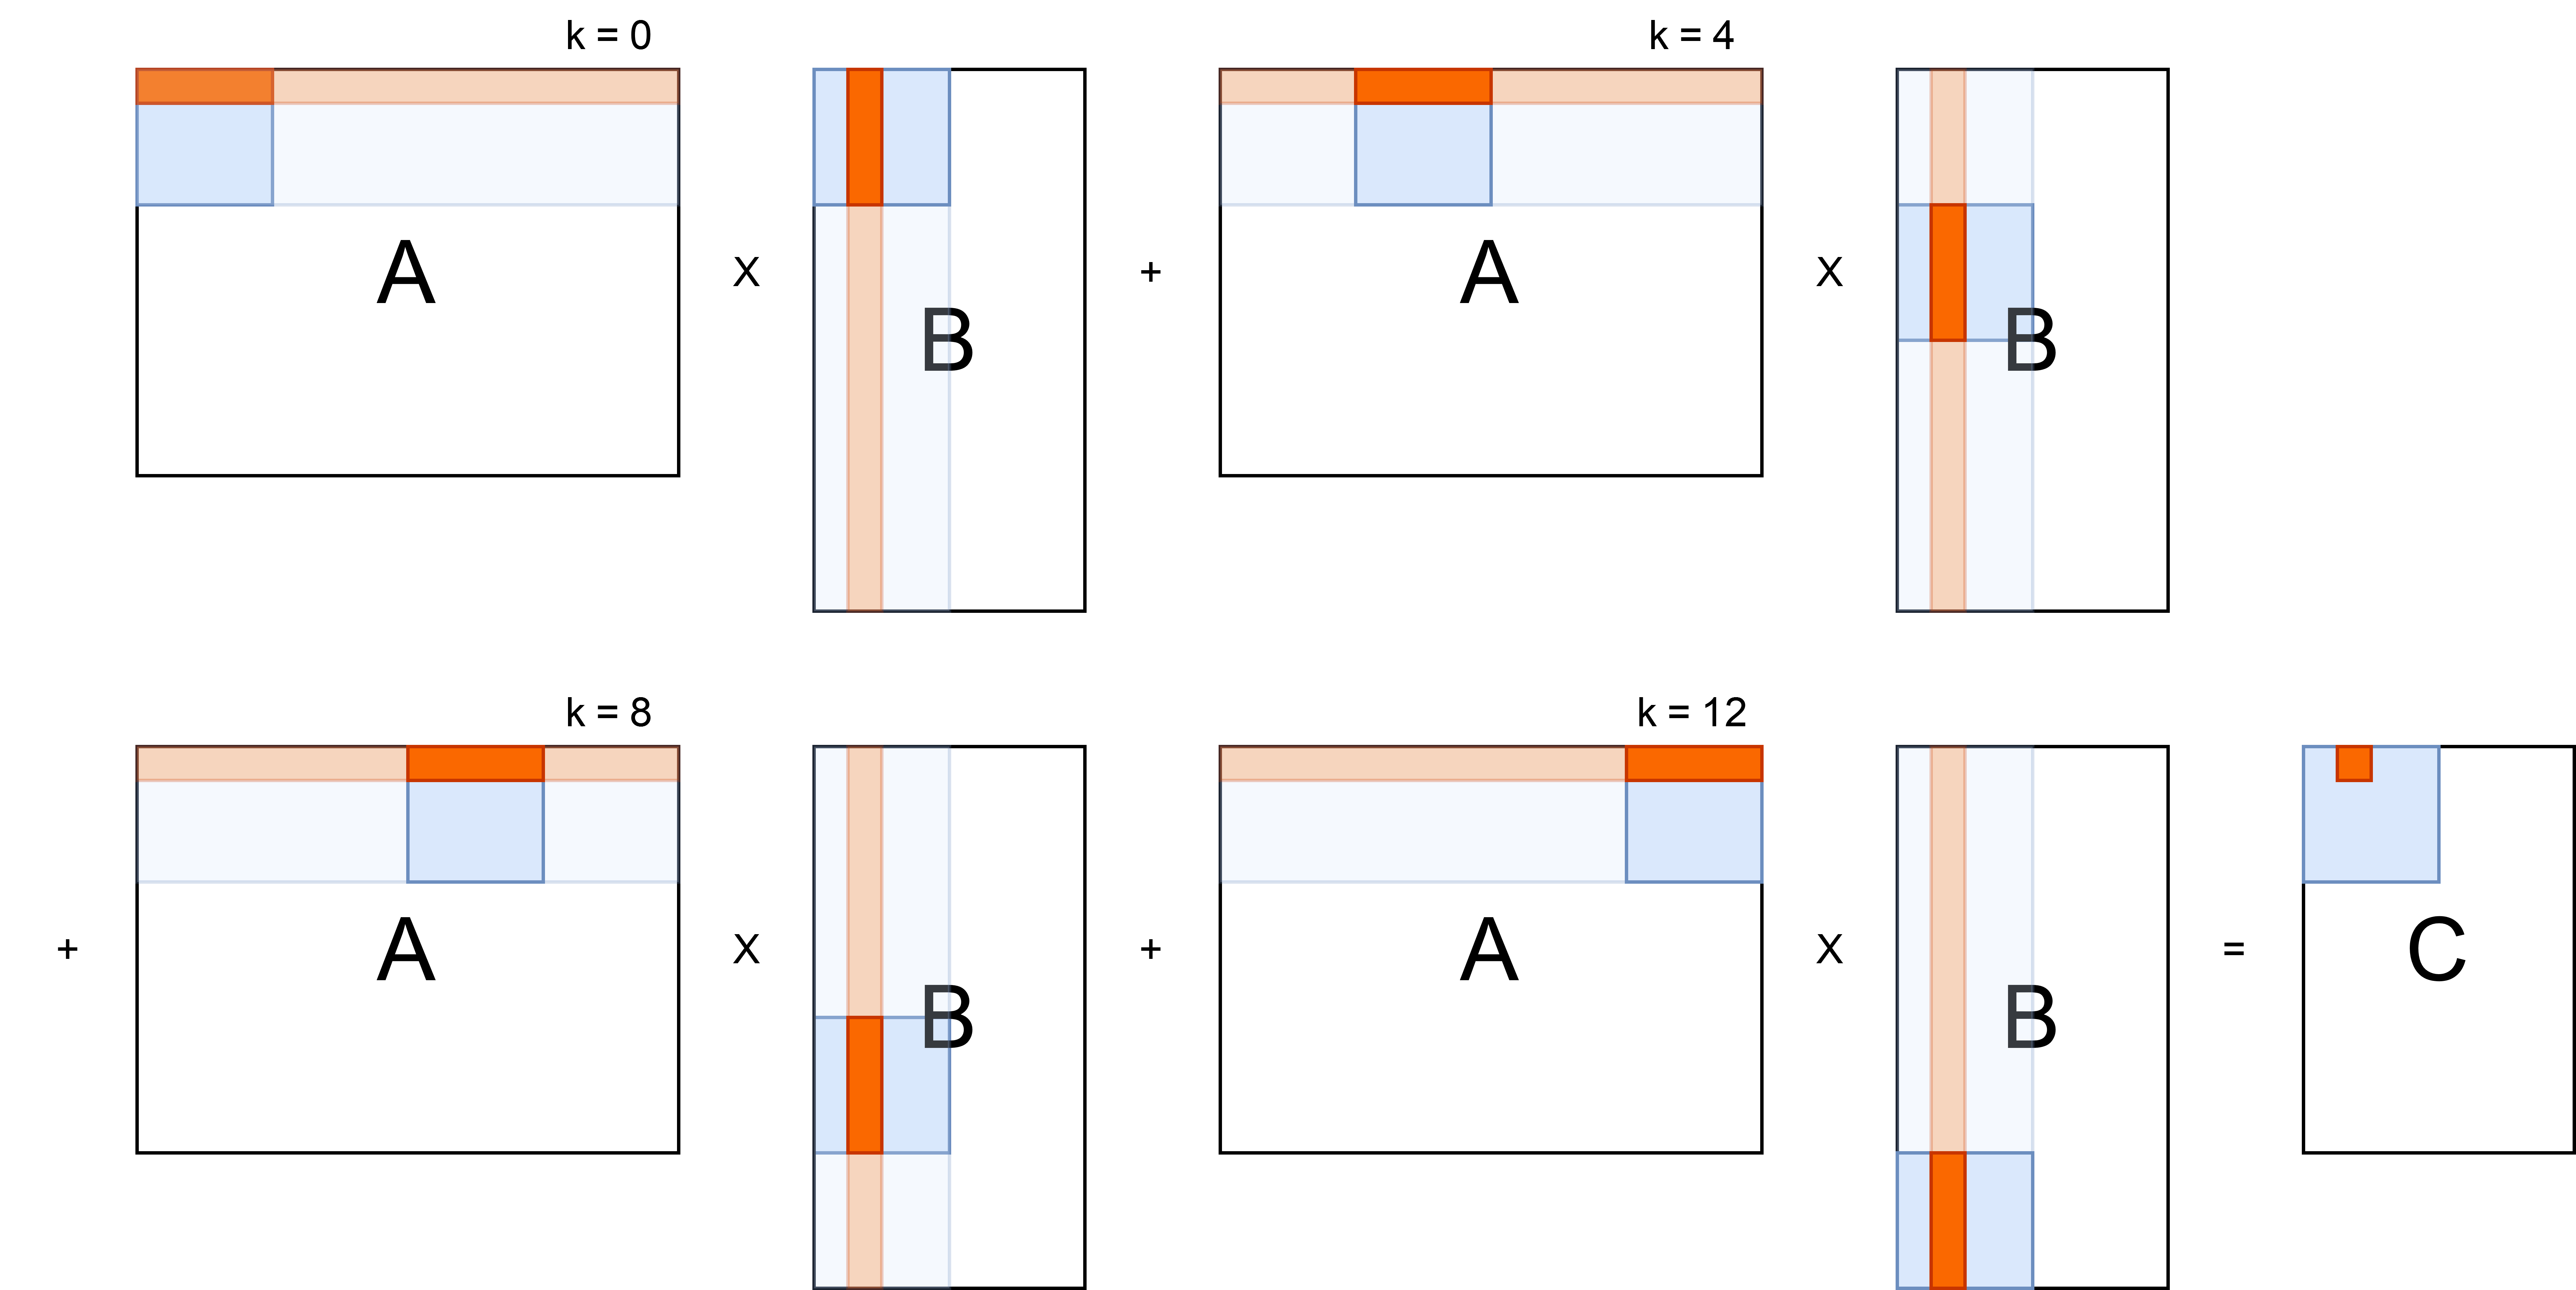
\includegraphics[width=\textwidth]{matmul/parallel_matmul.png}
  \caption{Visualization of the Vectorized Matrix Multiplication Algorithm. With one run of the $k$-loop, we compute one $4\times4$ submatrix of $C$ (marked in blue). The orange cells depict the calculation of a single element of $C$.}
  \label{fig:vectorizedmatrixmultiplication}
\end{figure}

\subsubsection{Handling Non-Multiples of 4}
The algorithm in Algorithm \ref{alg:vectorizedmatrixmultiplication} only works for matrices of which the dimensions are multiples of 4. Unfortunately, MEDS uses matrices of which the dimensions are usually not multiples of 4. To solve this problem, there are various approaches that we can take. An easy solution is to pad the matrices such that the dimensions become multiples of 4, but this would require additional memory and computation time.

Our solution to this problem is threefold, as there are three dimensions that can be non-multiples of 4: $m$, $o$, and $n$. We will handle each of these dimensions separately.
\begin{itemize}
  \item \textbf{Dimension $m$}:\\
  When $m$ is not a multiple of 4, we can use the normal approach until we reach the last multiple of 4. After this, when loading the submatrix of $A$, we load a $(m \mod 4) \times 4$ submatrix. Additionally, we only compute the dot products and store the results for the $m \mod 4$ rows of $C$ that are required.
  \item \textbf{Dimension $o$}:\\
  When $o$ is not a multiple of 4, we can use the normal approach until we reach the last multiple of 4. After this, when loading the submatrix of $B$, we load a $4 \times (o \mod 4)$ submatrix. The remaining lanes in the NEON registers containing $B_i$ are set to 0, making sure no incorrect values are added to $C$. When storing the results, we store only the first $o \mod 4$ columns of $C$.
  \item \textbf{Dimension $n$}:\\
  When $n$ is not a multiple of 4, we can use the normal approach until we reach the last multiple of 4. After this, we load only a $4 \times (n \mod 4)$ submatrix of $A$ and a $(n \mod 4) \times 4$ submatrix of $B$. When computing $C_i$, we skip the last $4 - (n \mod 4)$ multiplications and additions.
\end{itemize}
It is also possible for multiple of these dimension to be non-multiples of 4 at the same time. In this case, we can combine the approaches described above.

\subsubsection{Implementation}
The actual implementation of Algorithm \ref{alg:vectorizedmatrixmultiplication} combined with the handling of non-multiples can be done in multiple ways. As the resulting algorithm becomes quite complex, we figured that the C compiler might not be able to optimize the code as well as we can. Therefore, we have decided to implement a Python script\footnote{\url{https://github.com/MeItsLars/MEDS-ARMv8-optimization-thesis/blob/main/opt-low-level/src/asm/matmul/generate\_matmul\_asm.py}} that generates optimized ARMv8 assembly code. The script generates a specialized assembly function for each set of input dimensions that are used in MEDS.

\subsubsection{Minimum Cycle Bound}
In order to understand the performance of our optimized matrix multiplication algorithm, we need to find a minimum bound on the number of cycles that the algorithm will take to execute. In order to do this, we will establish a minimum bound on the number of instructions that the algorithm uses.

A very crude minimum cycle bound on the naive algorithm (see Algorithm \ref{alg:medsmatrixmultiplication}) can be established by counting the number of arithmetic operations required:
\begin{itemize}
  \item $m \cdot o \cdot n$ multiplications and additions
  \item $m \cdot o$ modulo operations
\end{itemize}
The `multiply-accumulate' operation is a single instruction on ARMv8, and modular reduction can be done in 5 instructions (see Section \ref{sec:barrettreduction}). This means that we can establish a minimum bound of $m \cdot o \cdot n + m \cdot o \cdot 5$ on the number of arithmetic instructions required for the naive algorithm. Any algorithm that follows this structure will require at least this number of instructions to execute, divided by the parallelization factor of that algorithm.

A more accurate minimum cycle bound can be established by looking at the number of instructions required for the vectorized algorithm (see Algorithm \ref{alg:vectorizedmatrixmultiplication}). This algorithm obtains a speedup because of two factors:
\begin{itemize}
  \item The NEON unit is able to perform operations in parallel.
  \item As we compute the result for a $4\times4$ submatrix of $C$ at the same time, we are able to use the same input value 4 times, reducing the number of loads required.
\end{itemize}
The number of instructions required for the vectorized algorithm can be calculated as follows:
\begin{itemize}
  \item $\frac{1}{4}m \cdot \frac{1}{4}o \cdot \frac{1}{4}n \cdot 4$ loads of $A$
  \item $\frac{1}{4}m \cdot \frac{1}{4}o \cdot \frac{1}{4}n \cdot 4$ loads of $B$
  \item $\frac{1}{4}m \cdot \frac{1}{4}o \cdot \frac{1}{4}n \cdot 4 \cdot 4$ multiply-accumulate operations
  \item $\frac{1}{4}m \cdot \frac{1}{4}o \cdot 4$ reductions
  \item $\frac{1}{4}m \cdot \frac{1}{4}o \cdot 4$ stores
\end{itemize}
Given that reduction takes 5 cycles and the remaining operations take 1 cycle, we establish a minimum bound of $\frac{1}{4}m \cdot \frac{1}{4}o \cdot \frac{1}{4}n \cdot 4 \cdot (1 + 1 + 4) + \frac{1}{4}m \cdot \frac{1}{4}o \cdot 4 \cdot (1 + 5) = \frac{1}{16}mo(6n + 24)$ cycles.

\subsection{Matrix Systemization}
\label{sec:matrixsystemization}
\todo[inline]{Change this section so it first gives a recap of what matrix systemization is, then discusses the optimization approach.}
\todo[inline]{The systemized forms (REF and RREF) should not be explained in this section but in the background section. Add references to Echelon?}
Matrix systemization is responsible for converting a matrix $A \in \mathbb{F}_{4093}^{m \times n}$ over the finite field $\mathbb{F}_{4093}$ into a systemized form. In MEDS, the systemized form $A' \in \mathbb{F}_{4093}^{m \times n}$ of a matrix $A \in \mathbb{F}_{4093}^{m \times n}$ can take two forms:
\begin{itemize}
  \item \textbf{REF}:\\
  $A'$ is in row-echelon form (REF), with the additional property that the leading coefficient of row $i$ is in column $i$.
  \item \textbf{RREF}:\\
  $A'$ is in reduced row-echelon form (RREF), with the additional property that the first $m \times m$ submatrix of $A'$ is the identity matrix.
\end{itemize}

The algorithm used in MEDS to systemize a matrix is a Gaussian elimination algorithm with some extra properties. The algorithm is implemented such that it runs in constant time, meaning that the execution time is the same for all matrices of equal size. Additionally, the algorithm contains some functionality that swaps rows and/or columns of the matrix to ensure that the leading coefficient of a row is not 0. The algorithm is is depicted in Algorithm \ref{alg:systemizer} (Appendix \ref{app:supplementalalgs}).

\subsubsection{Optimization}
\label{sec:matrixsystemizationoptimization}
We will optimize the matrix systemization algorithm by applying vectorization to the loops in the algorithm. Contrary to the matrix multiplication algorithm, we cannot easily parallelize the main $r$-loop in the algorithm, as the starting values of subloops depend on the (changing) value of $r$. This structure makes parallelization over the $r$-loop impossible. Instead, we will optimize each inner loop separately by applying a parallelization technique tailored to the specific inner loop.

For all nested loops, we will apply parallelization to the innermost loop. In the systemization algorithm, this loop is always the easiest to parallelize, as it accesses matrix elements that are stored next to each other in memory. Each input matrix element is stored in a 12-bit field element, which fits into a 16-bit register. This means that we can compute 8 elements at the same time using 128-bit NEON registers.

Unfortunately, we are unable to use a full 8-way vectorization for all loops, as the algorithm uses multiplication operations. When multiplying two 16-bit values, the result is a 32-bit value, of which we can not store 8 in a 128-bit NEON register. We can work around this issue by using the \texttt{umull} instruction to multiply the lower 4 16-bit values of two registers and the \texttt{umull2} instruction to multiply the upper 4 16-bit values of two registers. After reducing both results, we can use the \texttt{uzp1} operation to combine the results back into a single 128-bit register.

\subsubsection{Handling Non-Multiples of 8}
\label{sec:matrixsystemizationnonmultiples}
The inner loops that we are optimizing usually do not loop over a dimension that is a multiple of 8. To handle this, we use the following approach:
\begin{enumerate}
  \item While at least 8 elements are left to process, use the 8-way vectorization approach.
  \item After this, if there are at least 4 elements left to process, use one iteration of a 4-way vectorized approach.
  \item After this, use a non-vectorized approach for any remaining elements (maximum 3).
\end{enumerate}

\subsubsection{Implementation}
As with the matrix multiplication algorithm, the resulting systemization algorithm becomes quite complex. Although it can be implemented with NEON intrinsics, we opted for the faster approach of generating optimized ARMv8 assembly code using a Python script\footnote{\url{https://github.com/MeItsLars/MEDS-ARMv8-optimization-thesis/blob/main/opt-low-level/src/asm/systemizer/generate\_systemizer\_asm.py}}. The script generates a specialized assembly function for each set of input dimensions that are used in MEDS.

\subsubsection{Minimum Cycle Bound}
\todo[inline]{It's quite difficult to establish a good minimum bound on Matrix Systemization, but I will try to do it.}

\subsection{System Solving}
\label{sec:systemsolving}
In all three operations of MEDS, the \texttt{solve\_opt} function is used to solve a system of linear equations over the finite field $\mathbb{F}_{4093}$. The system that needs to be solved is constructed in a very specific way, which allows for a more efficient method of solving it (as opposed to using a more general algorithm like Gaussian elimination). Even though this more efficient method is used, the function still takes up a significant amount of time in the MEDS implementation.

% Majority of time is spent on two tripple-nested loops
Unfortunately, the function is also extremely large, with the reference code containing over 300 lines of code, making it very tedious to optimize the function as a whole. Instead, we profiled the function and found that the majority of the time of this function ($\pm 88 \%$\todo{Update measurement}) is spent on two relatively small tripple-nested loops, while the remainder of the time ($\pm 12 \%$\todo{Update measurement}) is spent on all other parts of the function combined. Therefore, we have decided to focus on optimizing these two loops. Both loops have the exact same structure, so we will only discuss the optimization of the first loop. This loop is shown in Algorithm \ref{alg:systemsolving1}.

\begin{algorithm}
  \caption{System Solving: Time-consuming loop 1}
  \label{alg:systemsolving1}
  \lstinputlisting[language=C, style=CStyle]{code/solve_opt_loop1.c}
\end{algorithm}

\subsubsection{Optimization}
\label{sec:systemsolvingoptimization}
Fortunately, the loop structure of the time-consuming loops in the algorithm is very suitable for vectorization. This has the negative consequence that the C compiler might already have optimized the loops to a degree that we cannot improve upon. Nevertheless, we will try to optimize the loops by applying vectorization to the innermost loop, which always loops from $0$ to $\texttt{MEDS\_m}$.

As the field elements are stored in 16 bits, we are able to compute 8 elements at the same time using 128-bit NEON registers. Therefore, we will compute the results for 8 values of $r$ at the same time. We start by loading \texttt{tmp1}, which gives us a small problem, as these 8 values are not stored next to each other in memory. Therefore, we load these values using normal load instructions and store them in a 128-bit NEON register. The remaining loads and stores can be done using vectorized instructions as those values are stored next to each other in memory.

Just like with matrix systemization, we are unable to use a full 8-way vectorization as the algorithm uses multiplication instructions, which result in 32-bit values. We apply the same approach as with matrix systemization to work around this issue, see Section \ref{sec:matrixsystemizationoptimization}.

\subsubsection{Handling Non-Multiples of 8}
Also like with matrix systemization, the number of elements that need to be processed is usually not a multiple of 8. We use the same approach as with matrix systemization to handle this issue (see Section \ref{sec:matrixsystemizationnonmultiples}), meaning we decrease the parallelization factor to 4 and 1 when there are not enough elements left to process.

\subsubsection{Implementation}
As the \texttt{solve\_opt} function is very large, we have decided not to implement the full function in ARMv8 assembly. This presented us with two options: either we use NEON intrinsics to parallelize the two time-consuming loops, or we write (a script that generates) ARMv8 assembly code for the two time-consuming loops. As the loops themselves are not very complex, we have decided to use NEON intrinsics to parallelize them, under the assumption that the assembly variant would not be much faster. Exploring the assembly-based optimization of these loops and the full function is left as future work\todo{Reference to section}.

The optimized C code with NEON intrinsics is quite elaborate, so we will not show it here. Instead, we refer to the code in the code repository\footnote{\url{https://github.com/MeItsLars/MEDS-ARMv8-optimization-thesis/blob/main/opt-low-level/src/util.c}}.

\subsubsection{Minimum Cycle Bound}
\todo[inline]{It's not possible to give a good minimum cycle bound on the entire System Solving algorithm, but it should be possible to give a cycle bound on these two loops. I'm not yet sure if this is necessary.}

\section{High-Level Optimization}
\label{sec:highleveloptimization}
The high-level optimization approach focuses on optimizing the MEDS implementation by parallelizing over the challenge space. MEDS uses a large number ($t$) of challenges and commitments in both signing and verification, which are all computed independently in a for-loop. Additionally, the computation for each commitment is exactly the same for signing and very similar for verification. This means that we can parallelize the computation of the commitments for each challenge.

Before we can parallelize the computation of the commitments, we need to determine the number of commitments that we will compute in parallel. The commitment computation is executed over $\mathbb{F}_{4093}$, which means that the field elements can be stored in 12 bits (which fits in a 16-bit register). This means that we can store up to 8 field elements in a single 128-bit NEON register. From this, there are two possible parallelization factors we can consider.
\begin{enumerate}
  \item \textbf{4-Way Parallelization}:\\
  Nearly all operations on field elements allow the values to stay in 16-bit registers. An exception is multiplication: the result of a multiplication of two field elements is a 24-bit value, which fits in a 32-bit register. This means that we can compute 4 multiplications at the same time using 128-bit NEON registers. Because of this limitation, we can choose to compute 4 commitments at a time.
  \item \textbf{8-Way Parallelization}:\\
  We can work around the multiplication limitation by using instructions such as \texttt{umull} and \texttt{umull2} to multiply the lower and upper 4 values (respectively) of two 128-bit NEON registers, after which we can reduce the results and combine them back into a single 128-bit register. Using this technique, we can compute 8 commitments at the same time.
\end{enumerate}
Our initial implementation uses 4-way parallelization, as this is the easiest to implement. We will explore the 8-way parallelization as future work\todo{Reference to section}.

In this section, we will discuss the high-level optimization of the MEDS implementation. We will first discuss the alterations that need to be made to the underlying datatypes and supplemental algorithms to allow for high-level parallelization in Section \ref{sec:highleveldataalgorithms}. Next, we will discuss the actual parallelization of the commitment computations in Section \ref{sec:commitmentparallelization}. Finally, we will discuss the limitations of the high-level optimization approach in Section \ref{sec:highlevellimitations}.

\subsection{Parallelization of Datatypes and Supplemental Algorithms}
\label{sec:highleveldataalgorithms}
In the reference implementation of MEDS, the main datatypes used are defined as follows:
\begin{verbatim}
  #define GFq_t uint16_t
  #define pmod_mat_t GFq_t
\end{verbatim}
These two datatypes represent a field element and a matrix element, respectively. Matrices are stored as one-dimensional arrays in row-major order, and are passed to functions using pointers to a \texttt{pmod\_mat\_t}.

In order to parallelize the algorithms that use these datatypes, we will adjust the datatypes such that they represent multiple field/matrix elements at the same time. In our implementation, we add a \texttt{vec\_16x4.h} file\footnote{\url{https://github.com/MeItsLars/MEDS-ARMv8-optimization-thesis/blob/main/opt-high-level/include/vec\_16x4.h}} containing these new datatypes, which are defined as follows:
\begin{verbatim}
  #define GFq_vec_t uint16x4_t
  #define pmod_mat_vec_t GFq_vec_t
\end{verbatim}
These two datatypes represent 4 field elements and 4 matrix elements, respectively. By passing these datatypes to a modified version of a function, we can compute the function output for 4 commitments at the same time.

Additionally, we will define a wide range of functions that operate on these vectorized datatypes in the \texttt{vec\_16x4.h} file. Examples of such definitions include:
\begin{verbatim}
  #define ADD_VEC(a, b) vaddl_u16(a, b)
  #define MUL_VEC(a, b) vmull_u16(a, b)
  #define OR_VEC(a, b) vorr_u16(a, b)
\end{verbatim}
The main advantage of this approach is that the entire high-level-optimized MEDS implementation can easily be converted to use a different CPU architecture (that supports vectorization) such as AVX512 \cite{intel-avx512} simply by changing the definitions in the \texttt{vec\_16x4.h} file.

\subsubsection{Supplemental Algorithms}
\label{sec:suppalgorithmsparallelization}
In order to parallelize the commitment computations, we need to modify the supplemental algorithms that are used in the MEDS implementation. In the reference implementation, these algorithms perform operations for matrices or values that belong to a single commitment. We need to modify these algorithms such that they can perform operations for multiple commitments at the same time. The following algorithms need to be modified:
\begin{enumerate}
  \item \textbf{Matrix Multiplication}: \texttt{pmod\_mat\_mul}\\
  Responsible for multiplying two matrices over the finite field $\mathbb{F}_{4093}$.
  \item \textbf{Matrix Systemization}: \texttt{pmod\_mat\_syst\_ct\_partial\_swap\_backsub}\\
  Responsible for converting a matrix into a systemized form (Algorithm \ref{alg:systemizer}, Appendix \ref{app:supplementalalgs}).
  \item \textbf{Field Inversion}: \texttt{GF\_inv}\\
  Responsible for inverting a field element over the finite field $\mathbb{F}_{4093}$.
  \item \textbf{Matrix Inversion}: \texttt{pmod\_mat\_inv}\\
  Responsible for inverting a matrix over the finite field $\mathbb{F}_{4093}$.
  \item \textbf{System Solving}: \texttt{solve\_opt}\\
  Responsible for solving a system of linear equations over the finite field $\mathbb{F}_{4093}$.
  \item \textbf{Applying the $\pi$ Function}: \texttt{pi}\\
  Responsible for applying the $\pi$ function (Algorithm \ref{alg:medspifunction}, Appendix \ref{app:supplementalalgs}) to a pair of matrices.
  \item \textbf{Applying the SF Function}: \texttt{SF}\\
  Responsible for applying the SF function (Algorithm \ref{alg:medssffunction}, Appendix \ref{app:supplementalalgs}) to a matrix.
\end{enumerate}
Each of these algorithms will be modified to work with the vectorized datatypes defined in the \texttt{vec\_16x4.h} file. These algorithms will then be plugged into the MEDS implementation, which will be modified to compute multiple commitments at the same time.

To give a brief overview of the modifications that need to be made to these algorithms, we will provide an example for the matrix multiplication algorithm. The reference matrix multiplication algorithm is shown in Algorithm \ref{alg:medsmatrixmultiplication} (Appendix \ref{app:supplementalalgs}). The C code for this algorithm is shown in Algorithm \ref{alg:medsmatrixmultiplicationc}. The modified matrix multiplication algorithm is shown in Algorithm \ref{alg:medsmatrixmultiplicationvec}. Both algorithms are slightly simplified for the sake of readability.

\begin{algorithm}
  \caption{Matrix Multiplication (Non-Vectorized)}
  \label{alg:medsmatrixmultiplicationc}
  \lstinputlisting[language=C, style=CStyle]{code/matrix_multiplication.c}
\end{algorithm}

\begin{algorithm}
  \caption{Matrix Multiplication (Vectorized for 4 commitments)}
  \label{alg:medsmatrixmultiplicationvec}
  \lstinputlisting[language=C, style=CStyle]{code/matrix_multiplication_vec.c}
\end{algorithm}

As can be seen from the code, the vectorized version is essentially the same as the non-vectorized version, but with certain operations altered so they work with the vectorized datatypes and functions defined in the \texttt{vec\_16x4.h} file. The same approach is used for all other supplemental algorithms that require parallelization, their modified implementations can be found in the code repository\footnote{\url{https://github.com/MeItsLars/MEDS-ARMv8-optimization-thesis/tree/main/opt-high-level/src}}.

\subsection{Parallelization of Commitment Computations}
\label{sec:commitmentparallelization}
Using the modified datatypes and supplemental algorithms, we can parallelize the computation of the commitments in MEDS. As can be seen in the algorithms for both signing (Algorithm X\todo{Update}) and verification (Algorithm X\todo{Update}), the computation of the commitments is done in a for-loop that loops from $0$ to $t$. As the generation of a commitment can fail (for example, when a randomly generated matrix is not invertible), the generation of a particular commitment is done in a while-loop that runs until the commitment is succesfully generated. This is why the signing and verification code exhibits the following structure:
\begin{verbatim}
  // Initial definitions and loading
  for (int i = 0; i < t; i++) {
    while (1) {
      // Compute commitment
      if (commitment is computed) {
        break;
      }
    }
  }
  // Final operations
\end{verbatim}
This structure introduces a problem if we want to parallelize the computation of the commitments. We can't simply parallelize the for-loop to use $\frac{t}{4}$ iterations, as the while loop might run for a different number of iterations for each commitment. Additionally, although the computation of two different commitments is independent, the computation of the same commitment (after a failure) is dependent on the previous computation of that commitment. This means that we also can't parallelize the while-loop.

\subsubsection{Optimization}
\label{sec:commitmentparallelizationoptimization}
We can overcome the aforementioned problems by using a different approach to parallelize the commitment computations. Instead of finishing the computation for a commitment before moving on to the next, we will start by running the first computation attempt for each commitment. If a computation fails, we will store the necessary information to retry the computation later. After the first computation attempt for all commitments is done, we will run the second computation attempt for all commitments that failed the first time. This process is repeated until all commitments are successfully computed. This approach is inspired by X\todo{Cite existing Git}. It is suitable for parallelization and has the following structure:
\begin{verbatim}
  // Initial definitions and loading
  while (there are uncomputed/failed commitments) {
    // 1. Load data for next 4 uncomputed/failed commitments
    // 2. Compute these commitments in parallel
    // 3(a). Store results for successful commitments
    // 3(b). Store information for failed commitments
  }
  // Final operations
\end{verbatim}
Of course, this introduces some overhead, as steps 1 and 3 in the structure above can not be parallelized and take slightly more time than their equivalent in the reference implementation. However, the parallelization of step 2 will result in a significant speedup, as the computation of the commitments itself is by far the most time-consuming part of the MEDS implementation.

\subsubsection{Loading and Storing}
\label{sec:commitmentparallelizationloadingstoring}
As we are computing multiple commitments at the same time, we need to alter the way in which we load and store the data for these commitments. Specifically, we need to make sure that the data for each computation is loaded into the correct lanes of a set of NEON registers.
\todo[inline]{Check complete data loading situation. Do we really need `MEDS\_t $\ll$ 1'? Re-run benchmarks if changes are made.}

\subsubsection{Verification}
\todo[inline]{Briefly explain the slightly different situation for verification, where there are two options (re-generate commitment or use the information in the signature).}

\subsection{Limitations}
\label{sec:highlevellimitations}
\todo[inline]{Explain how this approach (possibly) experiences a lot of issues with caching, as the input is 4 times bigger than before.}

\section{Bitstream Filling}
\label{sec:bitstreamfilling}
After the commitments are computed, the resulting matrices are hashed, after which the hash output is converted into an array of $t$ challenges. The input to the hash function is an array of 8-bit unsigned integers. For the MEDS parameter sets that we consider, the matrix elements fit in 12 bits and are stored as 16-bit unsigned integers. This means that the 16-bit values need to be converted to 8-bit values before they can be hashed. Although this can be done by simply changing the pointer type (for C implementations), MEDS uses the more complex approach of only using the 12 least significant bits (which contain the field element) of each 16-bit value. These 12-bit values are concatenated into a bitstream which is then hashed.

The main advantage of this approach is that the number of 8-bit values that need to be hashed is reduced by a factor of $\frac{16}{12} = \frac{4}{3}$, lowering the number of calls to the hash function. However, it also comes with the disadvantage that the process of filling the bitstream is more complex and time-consuming than the alternative of changing the pointer type.

\subsection{Optimizing the Existing Approach}
The reference implementation\footnote{\url{https://github.com/MeItsLars/MEDS-ARMv8-optimization-thesis/blob/main/ref/src/bitstream.c}} for filling the bitstream is generalized to work with up to 32 bits per value and therefore has to keep track of and update the current bit position in the bitstream. This means that we can save some time by using a specialized approach for filling bitstreams with 12-bit values.

Our optimization relies on the observation that two 12-bit values can be converted to three 8-bit values (which are required by the hash function) using a few simple bitwise operations. A conceptual pseudocode implementation of this approach is shown in Algorithm \ref{alg:bitstreamfilling}. The actual implementation\footnote{\url{https://github.com/MeItsLars/MEDS-ARMv8-optimization-thesis/blob/main/opt-low-level/src/meds.c}} is a bit more complex as the structure of the input data is different and it needs to handle the case where the number of values is not a multiple of 2. The high-level variant\footnote{\url{https://github.com/MeItsLars/MEDS-ARMv8-optimization-thesis/blob/main/opt-high-level/src/vec\_16x4.c}} is also slightly different as it needs to parallelize this operation.

\begin{algorithm}
  \label{alg:bitstreamfilling}
  \caption{Bitstream Filling for 12-bit values}
  \begin{algorithmic}
    \State \textbf{Input:} $v$: array of $n$ 16-bit unsigned integers
    \State \textbf{Output:} $bs$: array of $\frac{3}{2}n$ 8-bit unsigned integers
    \State $bs \gets \text{empty array of size } \frac{3}{2}n$
    \State $i \gets 0$
    \For{$j \gets 0$ to $n$ in steps of 2}
      \State $v_1 \gets v[j]$
      \State $v_2 \gets v[j + 1]$
      \State $bs[i] \gets v_1 ~\&~ \texttt{0xFF}$
      \State $bs[i + 1] \gets (v_1 \gg 8) ~|~ ((v_2 ~\&~ \texttt{0xF}) \ll 4)$
      \State $bs[i + 2] \gets (v_2 \gg 4) ~\&~ \texttt{0xFF}$
      \State $i \gets i + 3$
    \EndFor
  \end{algorithmic}
\end{algorithm}

\subsection{Alternative Approach}
\todo[inline]{I performed a quick check to see if the alternative approach of changing the pointer type is faster. It turns out it is ever so slightly faster. If there is time left, I will implement this approach as well. Otherwise, I will leave it as future work.}

\section{Hash Structure}
\label{sec:hashfunctionoptimization}
The result of the computation of each commitment is a large matrix. To convert these commitments into a set of challenges (as is required by the Fiat-Shamir structure, see Section \ref{sec:fiatshamir}), the commitments are hashed (using the SHAKE256 hash function) into a single KECCAK state. This state is then converted into an array of $t$ challenges.

The commitment matrices are hashed in a sequential manner, meaning that to hash commitment $i$, we are dependent on the hash output of commitment $i - 1$. The structure of this hashing process is depicted in Figure \ref{fig:hashstructure}. In this figure, $\tilde{\textbf{G}}_i$ represents the commitment matrix for commitment $i$, converted such that it is stored in an array of $k(mn - k)$ unsigned 8-bit integers (see Section \ref{sec:parametersets} for values of $m$, $n$, and $k$). $\textit{Hash}_1$ represents a call to SHAKE256, which in turn calls the Keccak-f[1600] permutation until the entire input array is absorbed. $s_i$ represents the intermediate KECCAK state after hashing commitment $i$, where $s_0$ is 0. The resulting state $s_t$ is used to generate the array of challenges.

\begin{figure}
  \centering
  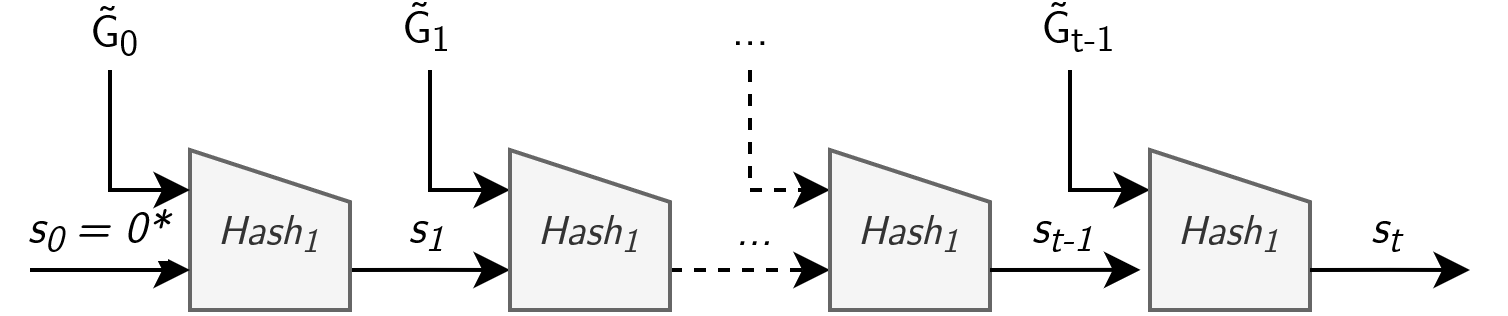
\includegraphics[width=\textwidth]{hash/hash_struct_seq.png}
  \caption{MEDS Commitment Hashing Structure.}
  \label{fig:hashstructure}
\end{figure}

The hashing process for a single commitment is already quite computationally expensive, as it requires $\frac{8 \cdot k(mn-k)}{1600}$ calls to the Keccak-f[1600] permutation (which operates on 1600 bits at a time). For parameter set 3 (see Section \ref{sec:parametersets}), this results in over 196 calls to the permutation. Additionally, the hashing process is not parallelizable because of the sequantial structure of the process. The profiling results (see Section \ref{sec:medsprofilingresults}) show that the hashing process takes up a little over 5\% of the total execution time of signing and verification, which makes it worthwhile to explore possible optimizations.

\subsection{Hash Structure Optimization}
There is little to no room for improvement in the actual SHAKE256 hash function, as it (and the underlying KECCAK permutation) is already widely studied and optimized. However, we can optimize the structure of the hashing process in such a way that we can compute the hashing result for multiple commitments in parallel. To do this, we need to alter the structure of the hashing process. This altered structure is depicted in Figure \ref{fig:hashstructureopt}. In this structure, the hashing structure is split into two stages:
\begin{enumerate}
  \item \textbf{Stage 1}: $\textit{Hash}_1$\\
  In the first stage, the commitment matrices are hashed into a set of intermediate states $i_0, i_1, \ldots, i_{t-1}$ using the same $\textit{Hash}_1$ function as in the original structure. This stage can be parallelized, as the hashing of each commitment no longer depends on other commitments.
  \item \textbf{Stage 2}: $\textit{Hash}_2$\\
  In the second stage, we combine the intermediate states $i_0, i_1, \ldots, i_{t-1}$ into a single state $s_t$ that we can use to generate the array of challenges. We do this by repeatedly applying the $\textit{Hash}_2$ function (which also calls SHAKE256) to the intermediate states and the running state $s$. This stage is once again sequential, but it only requires $t$ calls to the Keccak-f[1600] permutation.
\end{enumerate}
The resulting structure introduces a small amount of overhead, as stage 2 requires $t$ additional calls to the Keccak-f[1600] permutation. However, as stage 1 can now be parallelized, the overall execution time of the hashing process is expected to decrease.

\begin{figure}
  \centering
  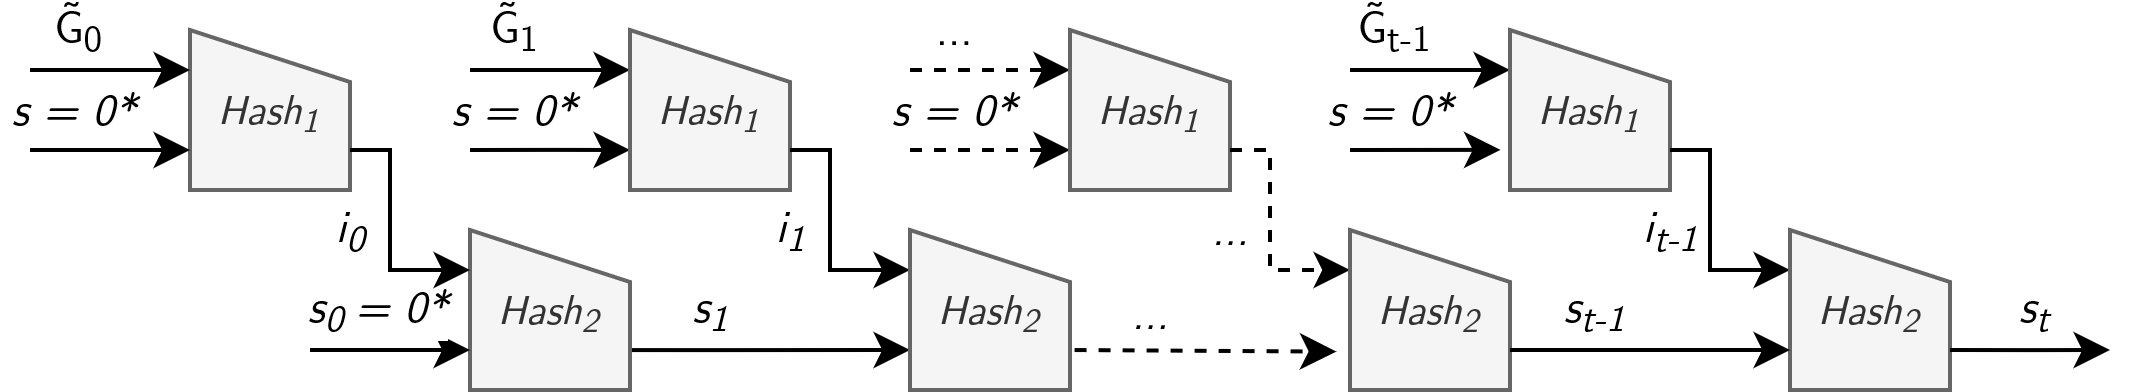
\includegraphics[width=\textwidth]{hash/hash_struct_par.png}
  \caption{Optimized MEDS Commitment Hashing Structure.}
  \label{fig:hashstructureopt}
\end{figure}

Unfortunately, the final state $s_t$ that the optimized structure generates is different from the final state that the original structure generates. This means that the resulting challenges will also be different between the two structures. Although this does not compromise the security of the scheme, it does meen that the optimized and reference implementations are not compatible with each other. Therefore, we leave this optimized hash structure as a suggested change to the MEDS scheme.

\subsection{Implementation}
The implementation of the optimized hash structure into the MEDS implementation is trivial, and requires only one important detail: a parallelized version of SHAKE256, optimized for the ARMv8 architecture. The extended KECCAK code package \cite{xkcp} does not contain optimized implementations of the Keccak-f[1600] permutation for ARMv8 (only for ARMv7). Fortunately, recent research by Becker and Kannwischer \cite{becker2022hybrid} has resulted in a large set of optimized implementations of the Keccak-f[1600] permutation for ARMv8 and various extensions of the ARMv8 architecture.

We have benchmarked these implementations on the Cortex-A72 and found that the \texttt{keccak\_f1600\_x4\_hybrid\_asm\_v3p}\footnote{\url{https://gitlab.com/arm-research/security/pqax/-/blob/master/asm/manual/keccak\_f1600/keccak\_f1600\_x4\_hybrid\_asm\_v3p.s}} optimized permutation (which is able to process 4 states in parallel) requires the lowest amount of cycles per state permutation. As the number of challenges $t$ is a multiple of 4 for all MEDS parameter sets that we consider, this means that we can easily plug this optimized permutation into the new hash structure.

\section{Non-Constant Time Implementations}
\label{sec:nonconstanttime}
% \todo[inline]{Explain the possibility of using non-constant time implementations for various functions in the verification phase.}
% - Use non-constant time implementations for various functions in the verification phase (both high and low level):
%   * Gaussian elimination 0 checks
%   * GF\_inv: use a lookup table
To prevent timing and cache-based side-channel attacks\todo{reference section}, it is important that the MEDS implementation is constant-time. However, this is only the case for the key generation and signing phases of MEDS. The verification phase is not required to be constant-time, as it operates only on public data. This means that we can use non-constant time code for the verification phase. In this section, we will list the functions that can be optimized using non-constant time implementations. The implementation of each optimization is slightly different for the low-level and high-level approach, but the idea is the same.

\subsection{Finite Field Inversion}
\todo[inline]{Mention the difficulty of speeding up the inversion of field elements in the systemizer algorithm (in some section).}
MEDS requires the inversion of field elements over the finite field $\mathbb{F}_{4093}$. The constant-time algorithm used in the reference implementation utilizes an optimal addition chain which takes a few hundred cycles to execute. However, as the number of possible field elements is limited to 4093, we can precompute the inverse of each field element and store it in a lookup table. This allows us to invert a field element simply by executing an array lookup, which takes only a few cycles to execute.

\subsection{Matrix Systemization}
During matrix systemization (shown in Algorithm \ref{alg:systemizer}), the algorithm spends some time on making sure the leading coefficient of each row is nonzero (it almost always is). As the implementation is constant time, this entire process is execute even if the leading coefficient is already nonzero. In a non-constant time implementation, we can add a check to see if the leading coefficient is zero, and if it is not, skip the entire process of making it nonzero.

\chapter{Results}
\label{ch:results}
In this chapter, we will present the results of the optimizations that we have performed on the MEDS implementation. We compiled the code using gcc (Debian 12.2.0-14) 12.2.0 with the \texttt{-O3} optimization flag. The code was compiled for the ARMv8 architecture and was ran on a Raspberry Pi 4 Model B with a 64-bit squad-core ARM Cortex-A72 CPU clocked at 1.5 GHz. In all tables and figures, the numbers shown represent the number of megacycles (MCycles, 1 MCycle = 1 million cycles) that that algorithm or function took to execute.

We will first look at the performance results of the three algorithms that were optimized specifically for the low-level approach in Section \ref{sec:resultslowlevel}. Next, we will do the same for the high-level approach in Section \ref{sec:resultshighlevel}. Finally, we will compare the overall performance of all implemented variants of the MEDS implementation in Section \ref{sec:overallperformance}.

\section{Low-Level Optimized Algorithms}
\label{sec:resultslowlevel}

\subsection{Matrix Multiplication}
\todo[inline]{Put bar plots in this section showing comparisons of the performance of traditional, optimized, and minimum cycle count matrix multiplication. Explain the results.}

\subsection{Matrix Systemization}
\todo[inline]{Put bar plots in this section showing comparisons of the performance of traditional, optimized, and minimum cycle count matrix systemization. Explain the results.}

\subsection{System Solving}
\todo[inline]{Put bar plots in this section showing comparisons of the performance of traditional, optimized, and minimum cycle count system solving. Explain the results.}

\section{High-Level Optimized Supplemented Algorithms}
\label{sec:resultshighlevel}
\todo[inline]{Compare results for the various algorithms that were optimized in the high-level approach with their reference implementations. Explain the results.}

\section{Overall Performance}
\label{sec:overallperformance}
We have benchmarked the performance of the MEDS for all combinations of the three relevant variables to consider:
\begin{itemize}
  \item \textbf{MEDS Parameter set}: We analyzed the performance for each of the three considered parameter sets: MEDS-21595, MEDS-55520, and MEDS-122000 (see Section \ref{sec:parametersets}).
  \item \textbf{Algorithm}: We tested each of the three signature algorithms: key generation, signing, and verification.
  \item \textbf{Implementation variant}: We tested all implementations: reference, low-level optimized, high-level optimized, low-level optimized with alternative hash structure, and high-level optimized with alternative hash structure.
\end{itemize}
MEDS was benchmarked for every possible combination of these variables, resulting in a total of 45 benchmarks. The result for each benchmark was obtained in the following way:
\begin{enumerate}
  \item 16 `warmup' runs were executed to ensure that the cache was filled with the necessary data and the branch predictor was optimized.
  \item 128 measurement runs were executed to obtain 128 measurements of the execution time of the algorithm.
  \item The final benchmark result was obtained by taking the median of the 128 measurements.
\end{enumerate}

The exact results of the benchmarks are shown in Table \ref{tab:overall_benchmark_results} in Appendix \ref{app:benchmark_results}. As the relative performance of the implementations is more important than the exact numbers, we depict the results in the form of bar charts in Figures \ref{fig:overal_performance_bar_chart_MEDS-21595} (MEDS-21595), \ref{fig:overal_performance_bar_chart_MEDS-55520} (MEDS-55520), and \ref{fig:overal_performance_bar_chart_MEDS-122000} (MEDS-122000).

\begin{figure}
  \centering
  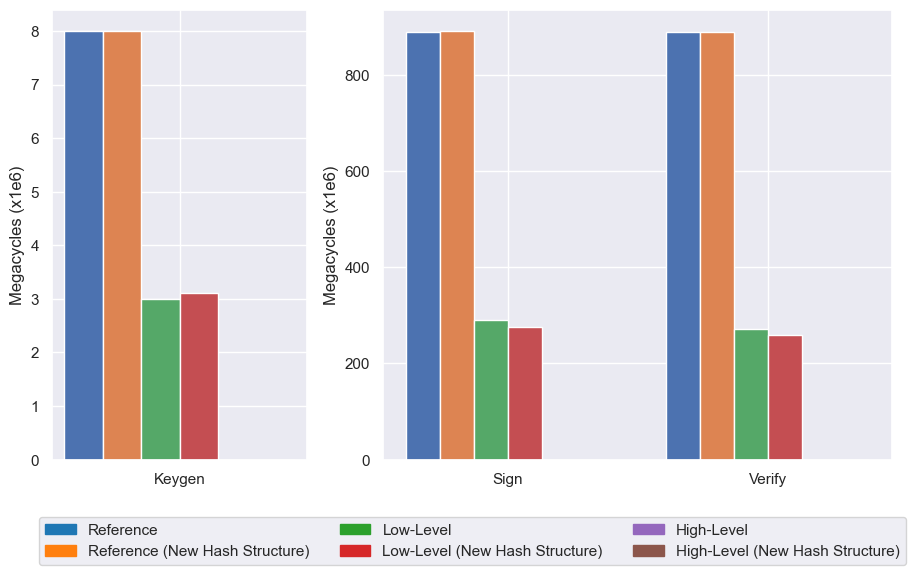
\includegraphics[width=\textwidth]{plots/barplot_MEDS-21595.png}
  \caption{Overall Performance of MEDS-21595 Variants.}
  \label{fig:overal_performance_bar_chart_MEDS-21595}
\end{figure}

\begin{figure}
  \centering
  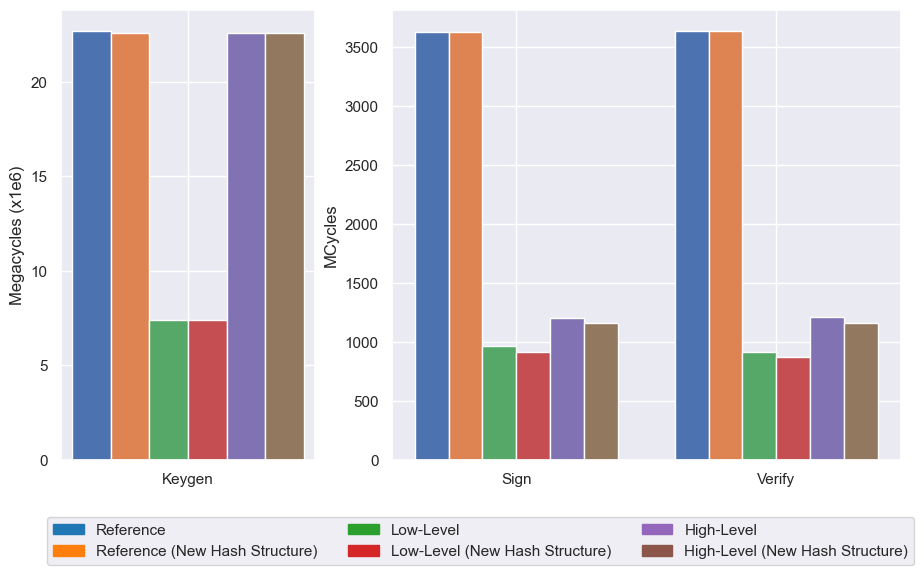
\includegraphics[width=\textwidth]{plots/barplot_MEDS-55520.png}
  \caption{Overall Performance of MEDS-55520 Variants.}
  \label{fig:overal_performance_bar_chart_MEDS-55520}
\end{figure}

\begin{figure}
  \centering
  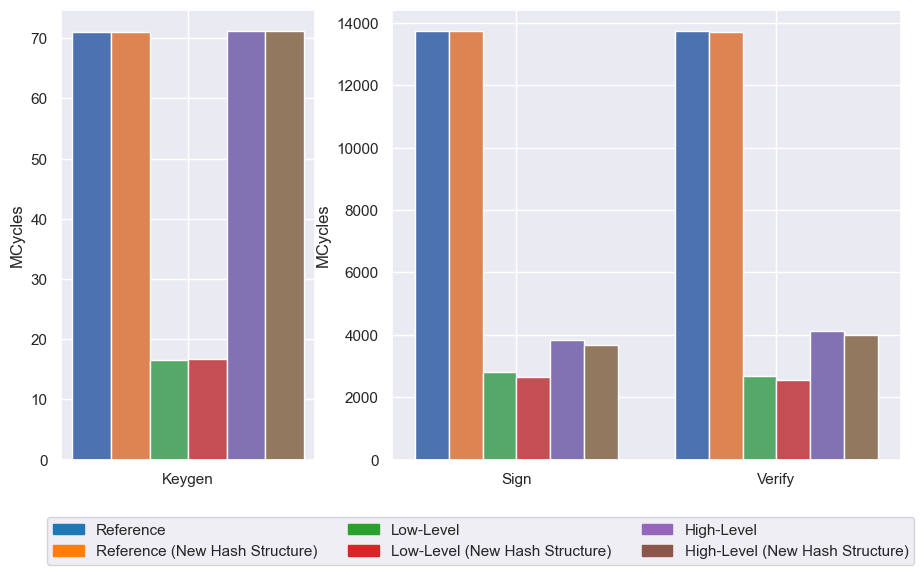
\includegraphics[width=\textwidth]{plots/barplot_MEDS-122000.png}
  \caption{Overall Performance of MEDS-122000 Variants.}
  \label{fig:overal_performance_bar_chart_MEDS-122000}
\end{figure}

\todo[inline]{Question to Peter and Simona: Is it a good idea to include an additional section in which I show profiling results for the optimized implementations? Here, I could show the distribution of cycles over the different functions (matrix multiplication, systemization, etc.) for the optimized implementations (possibly using piecharts).}

\todo[inline]{Question to Peter and Simona: Should I include a section in which I compare the performance of MEDS to the performance of other (similar) digital signature schemes?}

\chapter{Future work}
\label{ch:futurework}
\todo[inline]{The future work section contains all ideas for future work, but they have not yet been nicely formatted and explained.}
Future Work:
\begin{itemize}
  \item Explore the speedup possibilities on other ARM-based CPUs (such as Apple M1) which can possibly utilize larger caches and/or the better KECCAK primitives possible on Armv8.2-A (Cortex-A72 uses Armv8-A). See: \url{https://developer.arm.com/documentation/100076/0100/A64-Instruction-Set-Reference/A64-Cryptographic-Algorithms/A64-Cryptographic-instructions?lang=en}
  \item Perform high-level optimization for key generation (even though this is hard to do with our current parameter sets, as $s$ is always 2, limiting the parallelization possibilities).
  \item Optimize the `solve' method (for the low-level approach) using a pure-assembly approach.
  \item Analyse and optimize memory and power usage of the (optimized) MEDS implementation.
  \item Implement the optimized MEDS implementation on other CPU architectures that support SIMD instructions, such as AVX512.
\end{itemize}

Still plan to do myself:
\begin{itemize}
  \item Analyze the minimum time complexity of the low-level systemizer algorithm?
  \item Adust the 2 python generation files with an abstract file for clearity
  \item Cite ARM Calling Convention PDF \url{https://github.com/ARM-software/abi-aa/releases}
  \item Check possibilities for low-level matrix multiplication while working on 8x8 submatrices instead of 4x4 submatrices
  \item Check possibilities for high-level parallelization where 8 commitments are computed at the same time
  \item Check possibilities for ignoring bitstream setup before hashing into a challenge hash. Instead, we could just pass the entire commitment matrix into the hash function. This will require additional calls to the hash function, but it will skip the bitstream filling process.
  \item Assuming I get the Apple device in time, I will also benchmark the optimized MEDS implementation on that CPU.
\end{itemize}

\chapter{Conclusion}
\label{ch:conclusion}
From our results in Chapter \ref{ch:results} (and more specifically Section \ref{sec:overallperformance}), it is clear that our optimizations have resulted in a significant speedup of the MEDS implementation. The low-level optimization approach (as described in Section \ref{sec:lowleveloptimization}) has provided the highest speedup, with MEDS-21595 being sped up by a factor of 2.8, 3.5, and 3.7; MEDS-55520 by a factor of 3.1, 3.8, and 4.0; and MEDS-122000 by a factor of 4.2, 4.8, and 4.9, for key generation, signing, and verification, respectively. The high-level optimization approach (as described in Section \ref{sec:highleveloptimization}) has provided a smaller speedup due to the limitations in the cache size of the ARM Cortex-A72 CPU. This approach might provide a larger speedup on CPUs with larger cache sizes.

We present an alternative hash structure in Section \ref{sec:hashfunctionoptimization} that improves the performance of signing and verification by a small amount, at a negligible cost to the non-parallelized reference implementation. As this alternative hash structure results in different challenges and signatures, we leave it as a suggested change to the MEDS scheme.

We have shown that the MEDS implementation is very suitable for optimization using SIMD instructions. The achieved speedup on ARMv8 is significant, but we expect that future research can achieve even larger speedups on other architectures that support SIMD instructions, such as AVX512 \cite{intel-avx512}, on which 4 times as many field elements can be processed in parallel compared to ARMv8.

\todo[inline]{Add comparison information to other digital signature schemes?}

\bibliographystyle{plain}
\bibliography{bibliofile}

\appendix
\chapter{MEDS Algorithms}
\label{app:medsalgs}

\section{Notations and Functions}

\subsection{Notations}
In the algorithms in this appendix, we use the following notations in addition to the notations mentioned in Section \ref{sec:notations}:
\begin{itemize}
  \item $\ell_{x}$: The size of the variable $x$ in bytes.
  \item $\mathcal{B}^{x}$: The set of all byte strings of length $x$.
  \item $\sigma$: A seed used to generate random values.
  \item $\text{GL}_k(q)$: The set of all invertible $k \times k$ matrices over $\mathds{F}_q$.
  \item $b[i,j]$: The $j-i$ byte long substring of byte string $b$ starting at index $i$.
  \item $\textbf{A}[;i,j]$: The submatrix of $\textbf{A}$ that starts at column $i$ (inclusive) and ends at column $j$ (exclusive), containing all rows.
  \item $(x~|~y)$: The concatenation of byte strings $x$ and $y$.
\end{itemize}

\subsection{Functions}
In the algorithms in this appendix, we use the following functions (in order of appearance):
\begin{itemize}
  \item Randombytes($x$): Generates a random byte string of length $x$.
  \item ExpandSysMat($\sigma$): Generate a random systematic matrix from seed $\sigma$.
  \item XOF($\sigma$, $x$, $y$): Generates two random byte strings of length $x$ and $y$ from seed $\sigma$.
  \item ExpandInvMat($\sigma$, $k$): Generates a random invertible matrix of size $k \times k$ from seed $\sigma$.
  \item Solve($\textbf{G}$): Solves the system of linear equations represented by matrix $\textbf{G}$.
  \item SF($\textbf{G}$): Converts matrix $\textbf{G}$ to systematic form.
  \item Compress(G)($\textbf{A}$): Compresses matrix $\textbf{A}$ into a byte string.
  \item Decompress(G)($x$): Decompresses byte string $x$ into a matrix.
  \item SeedTree$_t(\rho, \alpha)$: \todo{Add description}
  \item ToBytes($x$, $y$): Converts $x$ to a byte string of length $y$.
  \item ExpandRndMat($\sigma$): Generates a random matrix from seed $\sigma$.
  \item H($x$): Hashes byte string $x$.
  \item ParseHash$_{s,t,w}(d)$: Parses hash $d$ into $t$ challenges that are smaller than $s$ each, where $w$ challenges are 0.
  \item SeedTreeToPath$_t(h_0, \ldots, h_{t-1}, \rho, \alpha)$: \todo{Add description}
  \item ParseSig($m_s$): Parses the signed message $m_s$ into its components.
  \item PathToSeedTree$_t(h_0, \ldots, h_{t-1}, p, \alpha)$: \todo{Add description}
\end{itemize}

\section{Key Algorithms}
\begin{algorithm}[H]
\caption{MEDS.KeyGen()}\label{alg:medskeygen}
\hspace*{\algorithmicindent} \textbf{Input:} -\\
\hspace*{\algorithmicindent} \textbf{Output:} public key $\textbf{pk} \in \mathcal{B}^{\ell_\textbf{pk}}$, secret key $\textbf{sk} \in \mathcal{B}^{\ell_\textbf{sk}}$
\begin{algorithmic}[1]
% Generate a random secret seed
\State $\delta \in \mathcal{B}^{\ell_\text{sec\_seed}} \gets \text{Randombytes}(\ell_\text{sec\_seed})$
% Generate random secret and public seed from the previously generated secret seed
\State $\sigma_{\textbf{G}_0} \in \mathcal{B}^{\ell_\text{pub\_seed}}, \sigma \in \mathcal{B}^{\ell_\text{sec\_seed}} \gets \text{XOF}(\delta, \ell_\text{pub\_seed}, \ell_\text{sec\_seed})$
% Generate a random matrix G_0 from the public seed
\State $\textbf{G}_0 \in \mathds{F}_q^{k \times mn} \gets \text{ExpandSysMat}(\sigma_{\textbf{G}_0})$
% Generate G_i for every s
\ForAll{$i \in \{1, \ldots, s - 1\}$}
    % Generate two new seeds from the current state of the secret seed and replace the current secret seed
    \State $\sigma_{\textbf{T}_i}, \sigma \in \mathcal{B}^{\ell_\text{sec\_seed}} \gets \text{XOF}(\sigma, \ell_\text{sec\_seed}, \ell_\text{sec\_seed})$
    % Generate a random invertible matrix T_i
    \State $\textbf{T}_i \in \text{GL}_k(q) \gets \text{ExpandInvMat}(\sigma_{\textbf{T}_i}, k)$
    % Compute G_0' = T_i * G_0
    \State $\textbf{G}_0' \in \mathds{F}_q^{k \times mn} \gets \textbf{T}_i \textbf{G}_0$
    % Solve system of equations to obtain A and B
    \State $\check{\textbf{A}}_i \in \mathds{F}_q^{m \times m} \cup \{\bot\}, \check{\textbf{B}}_i \in \mathds{F}_q^{n \times n} \cup \{\bot\} \gets \text{Solve}(\textbf{G}_0')$
    % Retry if there was no solution
    \If{$(\check{\textbf{A}}_i = \bot \textbf{ and } \check{\textbf{B}}_i = \bot) \textbf{ or } \check{\textbf{A}}_i \notin \text{GL}_m(q) \textbf{ or } \check{\textbf{B}}_i \notin \text{GL}_n(q)$}
        \State \textbf{goto} line 5
    \EndIf
    % Get A_i, A_i^-1, B_i, and B_i^-1 from the solution
    % Theoretically we don't need to rename these variables, but it is done for notation
    \State $\textbf{A}_i, \textbf{A}_i^{-1} \in \text{GL}_m(q) \gets \check{\textbf{A}}_i, \check{\textbf{A}}_i^{-1}$
    \State $\textbf{B}_i, \textbf{B}_i^{-1} \in \text{GL}_n(q) \gets \check{\textbf{B}}_i, \check{\textbf{B}}_i^{-1}$
    % Compute Gi
    \State $\textbf{G}_i \in \mathds{F}_q^{k \times mn} \gets \pi_{\textbf{A}_i, \textbf{B}_i}(\textbf{G}_0)$
    % Compute Compute T_i^-1 as a k*k submatrix of G_i
    \State $\textbf{T}_i^{-1} \in \mathds{F}_q^{k \times k} \gets \textbf{G}_i[;0,k-1]$
    % Convert Gi to systematic form
    \State $\textbf{G}_i \in \mathds{F}_q^{k \times mn} \cup \{\bot\} \gets \text{SF}(\textbf{G}_i)$
    % Retry if the matrix is not in systematic form
    \If{$\textbf{G}_i = \bot$}
        \State \textbf{goto} line 5
    \EndIf
    \EndFor
% Compute the pk from the data
\State $\text{pk} \in \mathcal{B}^{\ell_\textbf{pk}} \gets (\sigma_{\textbf{G}_0}~|~\text{CompressG}(\textbf{G}_1)~|~\ldots~|~\text{CompressG}(\textbf{G}_{s-1}))$
% Compute the sk from the data
\State $\text{sk} \in \mathcal{B}^{\ell_\textbf{sk}} \gets (\delta~|~\sigma_{\textbf{G}_0}~|~\text{Compress}(\textbf{A}_1^{-1})~|~\ldots~|~\text{Compress}(\textbf{A}_{s-1}^{-1})$\\
$\quad\quad\quad\quad\quad\quad\quad\quad\quad~|~\text{Compress}(\textbf{B}_1^{-1})~|~\ldots~|~\text{Compress}(\textbf{B}_{s-1}^{-1})$\\
$\quad\quad\quad\quad\quad\quad\quad\quad\quad~|~\text{Compress}(\textbf{T}_1^{-1})~|~\ldots~|~\text{Compress}(\textbf{T}_{s-1}^{-1}))$
% Return the public and secret key
\State \textbf{return} $\text{pk}, \text{sk}$
\end{algorithmic}
\end{algorithm}

\newpage

\begin{algorithm}[H]
\caption{MEDS.Sign()}\label{alg:medssign}
\hspace*{\algorithmicindent} \textbf{Input:} secret key $\textbf{sk} \in \mathcal{B}^{\ell_\textbf{sk}}$, message $m \in \mathcal{B}^{\ell_m}$\\
\hspace*{\algorithmicindent} \textbf{Output:} signed message $m_s \in \mathcal{B}^{\ell_\text{sig} + \ell_m}$
\begin{algorithmic}[1]
% Initialize parsing index
\State $f_\text{sk} \gets \ell_\text{sec\_seed}$
% Parse sigma_G_0 from the secret key
\State $\sigma_{\textbf{G}_0} \gets \text{pk}[f_\text{sk}, f_\text{sk} + \ell_\text{pub\_seed} - 1]$
% Construct G0
\State $\textbf{G}_0 \in \mathds{F}_q^{k \times mn} \gets \text{ExpandSysMat}(\sigma_{\textbf{G}_0})$
% Increment index; skip public seed and A and B?
\State $f_\text{sk} \gets f_\text{sk} + \ell_\text{pub\_seed} + (s - 1) \cdot (\ell_{\mathds{F}_q^{m \times m}} + \ell_{\mathds{F}_q^{n \times n}})$
% % Obtain all A_i from the secret key
% \ForAll{$i \in \{1, \ldots, s - 1\}$}
%     % Parse A_i from the secret key
%     \State $\textbf{A}_i^{-1} \in \mathds{F}_q^{m \times m} \gets \text{Decompress}(\text{sk}[f_\text{sk}, f_\text{sk} + \ell_{\mathds{F}_q^{m \times m}}])$
%     % Update the parsing index
%     \State $f_\text{sk} \gets f_\text{sk} + \ell_{\mathds{F}_q^{m \times m}}$
% \EndFor
% % Obtain all B_i from the secret key
% \ForAll{$i \in \{1, \ldots, s - 1\}$}
%     % Parse B_i from the secret key
%     \State $\textbf{B}_i^{-1} \in \mathds{F}_q^{n \times n} \gets \text{Decompress}(\text{sk}[f_\text{sk}, f_\text{sk} + \ell_{\mathds{F}_q^{n \times n}}])$
%     % Update the parsing index
%     \State $f_\text{sk} \gets f_\text{sk} + \ell_{\mathds{F}_q^{n \times n}}$
% \EndFor
% Obtain all T_i from the secret key
\ForAll{$i \in \{1, \ldots, s - 1\}$}
    % Parse T_i from the secret key
    \State $\textbf{T}_i^{-1} \in \mathds{F}_q^{k \times k} \gets \text{Decompress}(\text{sk}[f_\text{sk}, f_\text{sk} + \ell_{\mathds{F}_q^{k \times k}}])$
    % Update the parsing index
    \State $f_\text{sk} \gets f_\text{sk} + \ell_{\mathds{F}_q^{k \times k}}$
\EndFor
% Generate a random seed
\State $\delta \in \mathcal{B}^{\ell_\text{sec\_seed}} \gets \text{Randombytes}(\ell_\text{sec\_seed})$
% Generate a random tree seed and salt from the secret seed
\State $\rho \in \mathcal{B}^{\ell_\text{tree\_seed}}, \alpha \in \mathcal{B}^{\ell_\text{salt}} \gets \text{XOF}(\delta, \ell_\text{tree\_seed}, \ell_\text{salt})$
% Construct t commitment seeds from the tree seed
\State $\sigma_0, \ldots, \sigma_{t-1} \in \mathcal{B}^{\ell_\text{tree\_seed}} \gets \text{SeedTree}_t(\rho, \alpha)$
% Generate t commitments from the challenge seeds
\ForAll{$i \in \{0, \ldots, t - 1\}$}
    % Construct a commitment seed for the current commitment
    \State $\sigma'_i \in \mathcal{B}^{\ell_\text{salt} + \ell_\text{tree\_seed} + 4} \gets (\alpha~|~\sigma_i~|~\text{ToBytes}(2^{1 + \lceil \log_2(t) \rceil + i}, 4))$
    % Generate seeds based on the current commitment seed
    \State $\sigma_{\tilde{\textbf{M}}_i} \in \mathcal{B}^{\ell_\text{pub\_seed}}, \sigma_i \in \mathcal{B}^{\ell_\text{tree\_seed}} \gets \text{XOF}(\sigma'_i, \ell_\text{pub\_seed}, \ell_\text{tree\_seed})$
    % Generate matrix ~M_i <- c0 and c1 represent the linear combination of codewords
    \State $\tilde{\textbf{M}}_i \in \mathds{F}_q^{2 \times k} \gets \text{ExpandRndMat}(\sigma_{\tilde{\textbf{M}}_i})$
    % Compute C = ~M_i * G_0 <- C contains the two codewords C0 and C1
    \State $\textbf{C} \in \mathds{F}_q^{2 \times mn} \gets \tilde{\textbf{M}}_i \textbf{G}_0$
    % Solve the system of equations to obtain A and B
    \State $\widetilde{\textbf{A}}_i \in \mathds{F}_q^{m \times m} \cup \{\bot\}, \widetilde{\textbf{B}}_i \in \mathds{F}_q^{n \times n} \cup \{\bot\} \gets \text{Solve}(\textbf{C})$
    % Retry if there was no solution
    \If{$(\widetilde{\textbf{A}}_i = \bot \textbf{ and } \widetilde{\textbf{B}}_i = \bot) \textbf{ or } \widetilde{\textbf{A}}_i \notin \text{GL}_m(q) \textbf{ or } \widetilde{\textbf{B}}_i \notin \text{GL}_n(q)$}
        \State \textbf{goto} line 12 % 18?
    \EndIf
    % Compute G_i
    \State $\tilde{\textbf{G}}_i \in \mathds{F}_q^{k \times mn} \gets \pi_{\widetilde{\textbf{A}}_i, \widetilde{\textbf{B}}_i}(\textbf{G}_0)$
    % Convert G_i to systematic form
    \State $\tilde{\textbf{G}}_i \in \mathds{F}_q^{k \times mn} \cup \{\bot\} \gets \text{SF}(\tilde{\textbf{G}}_i)$
    % Retry if the matrix is not in systematic form
    \If{$\tilde{\textbf{G}}_i = \bot$}
        \State \textbf{goto} line 12 % 18?
    \EndIf
\EndFor
% Create hash
\State $d \in \mathcal{B}^{\ell_\text{digest}} \gets \text{H}(\text{Compress}(\tilde{\textbf{G}}_0[;k,mn-1])~|~\ldots$\\
$\quad\quad\quad\quad\quad\quad~~|~\text{Compress}(\tilde{\textbf{G}}_{t-1}[;k,mn-1])~|~m)$
% Parse challenges from the hash
\State $h_0, \ldots, h_{t-1} \in \{0, \ldots, s-1\} \gets \text{ParseHash}_{s,t,w}(d)$
% For each challenge, compute the response
\ForAll{$i \in \{0, \ldots, t - 1\}$}
    % Only for non-zero challenges
    \If{$h_i > 0$}
        % Compute response
        \State $\kappa_i \in \mathds{F}_q^{2 \times k} \gets \tilde{\textbf{M}}_i T_{h_i}^{-1}$
    \EndIf
\EndFor
% Construct seed tree paths
\State $p \in \mathcal{B}^{\ell_\text{path}} \gets \text{SeedTreeToPath}_t(h_0, \ldots, h_{t-1}, \rho, \alpha)$
% Return the signature
\State \textbf{return} $m_s \in \mathcal{B}^{w \cdot \ell_{\mathds{F}_q^{2 \times k}} + \ell_\text{path} + \ell_\text{digest} + \ell_\text{salt} + \ell_\text{m} = \ell_\text{sig} + \ell_\text{m}}$\\
$\quad\quad\quad\quad= (\kappa_0~|~\ldots~|~\kappa_{t-1}~|~p~|~d~|~\alpha~|~m)$
\end{algorithmic}
\end{algorithm}

\begin{algorithm}[H]
\caption{MEDS.Verify()}\label{alg:medsverify}
\hspace*{\algorithmicindent} \textbf{Input:} public key $\textbf{pk} \in \mathcal{B}^{\ell_\textbf{pk}}$, signed message $m_s \in \mathcal{B}^{\ell_\text{sig} + \ell_m}$\\
\hspace*{\algorithmicindent} \textbf{Output:} message $m \in \mathcal{B}^{\ell_m}$ or $\bot$
\begin{algorithmic}[1]
% Initialize parsing index
\State $\sigma_{\textbf{G}_0} \gets \text{pk}[0, \ell_\text{pub\_seed} - 1]$
% Construct G0
\State $\textbf{G}_0 \in \mathds{F}_q^{k \times mn} \gets \text{ExpandSysMat}(\sigma_{\textbf{G}_0})$
% Initialize parsing index
\State $f_\text{pk} \gets \ell_\text{pub\_seed}$
% Parse all G_i from the public key
\ForAll{$i \in \{1, \ldots, s - 1\}$}
    % Parse G_i from the public key
    \State $\textbf{G}_i \in \mathds{F}_q^{k \times mn} \gets \text{DecompressG}(\text{pk}[f_\text{pk}, f_\text{pk} + \ell_{\mathds{F}_q^{k \times mn}}])$
    % Update the parsing index
    \State $f_\text{pk} \gets f_\text{pk} + \ell_{G_i}$
\EndFor

% % Parse the path
% \State $p \in \mathcal{B}^{\ell_\text{path}} \gets m_s[\ell_\text{sig} - \ell_\text{digest} - \ell_\text{salt} - \ell_\text{path}, \ell_\text{sig} - \ell_\text{digest} - \ell_\text{salt} - 1]$
% % Parse the salt
% \State $\alpha \in \mathcal{B}^{\ell_\text{salt}} \gets m_s[\ell_\text{sig} - \ell_\text{digest} - \ell_\text{salt}, \ell_\text{sig} - \ell_\text{digest} - 1]$
% % Parse the digest
% \State $d \in \mathcal{B}^{\ell_\text{digest}} \gets m_s[\ell_\text{sig} - \ell_\text{digest}, \ell_\text{sig} - 1]$
% % Parse the message
% \State $m \in \mathcal{B}^{\ell_m} \gets m_s[\ell_\text{sig},]$
% % Compute the hash
% \State $h_0, \ldots, h_{t-1} \in \{0, \ldots, s-1\} \gets \text{ParseHash}_{s,t,w}(d)$

% Parse m_s
\State $p \in \mathcal{B}^{\ell_\text{path}}, \alpha \in \mathcal{B}^{\ell_\text{salt}}, d \in \mathcal{B}^{\ell_\text{digest}}, m \in \mathcal{B}^{\ell_m} \gets \text{ParseSig}(m_s)$
% Convert the path to seed tree seeds
\State $\sigma_0, \ldots, \sigma_{t-1} \in \mathcal{B}^{\ell_\text{tree\_seed}} \gets \text{PathToSeedTree}_t(h_0, \ldots, h_{t-1}, p, \alpha)$
% Loop through all t challenges
\ForAll{$i \in \{0, \ldots, t - 1\}$}
    \If{$h_i > 0$}
        % Non-zero challenges
        % Get kappa_i from the signature
        \State $\kappa_i \in \mathds{F}_q^{2 \times k} \gets m_s[i \cdot \ell_{\mathds{F}_q^{2 \times k}}, (i + 1) \cdot \ell_{\mathds{F}_q^{2 \times k}} - 1]$
        % Compute G0' = kappa * G[h_i]
        \State $\textbf{G}_0' \in \mathds{F}_q^{2 \times mn} \gets \kappa_i \textbf{G}_{h_i}$
        % Solve the system of equations to obtain A_hat and B_hat
        \State $\hat{\textbf{A}}_i \in \mathds{F}_q^{m \times m} \cup \{\bot\}, \hat{\textbf{B}}_i \in \mathds{F}_q^{n \times n} \cup \{\bot\} \gets \text{Solve}(\textbf{G}_0')$
        % Abort if there was no solution
        \If{$(\hat{\textbf{A}}_i = \bot \textbf{ and } \hat{\textbf{B}}_i = \bot) \textbf{or } \hat{\textbf{A}}_i \notin \text{GL}_m(q) \textbf{ or } \hat{\textbf{B}}_i \notin \text{GL}_n(q)$}
            \State \textbf{return} $\bot$
        \EndIf
        % Compute G_hat_i with pi
        \State $\hat{\textbf{G}}_i \in \mathds{F}_q^{k \times mn} \gets \pi_{\hat{\textbf{A}}_i, \hat{\textbf{B}}_i}(\textbf{G}_{h_i})$
        % Convert G_hat_i to systematic form
        \State $\hat{\textbf{G}}_i \in \mathds{F}_q^{k \times mn} \cup \{\bot\} \gets \text{SF}(\hat{\textbf{G}}_i)$
        % Abort if the matrix is not in systematic form
        \If{$\hat{\textbf{G}}_i = \bot$}
            \State \textbf{return} $\bot$
        \EndIf
    \Else
        % Zero challenges; we need to re-compute the G_i completely
        % Compute seed for the commitment
        \State $\sigma_i' \in \mathcal{B}^{\ell_\text{salt} + \ell_\text{tree\_seed} + 4} \gets (\alpha~|~\sigma_i~|~\text{ToBytes}(2^{1 + \lceil \log_2(t) \rceil + i}, 4))$
        % Generate seeds based on the current commitment seed
        \State $\sigma_{\hat{M}_i} \in \mathcal{B}^{\ell_\text{pub\_seed}}, \sigma_i \in \mathcal{B}^{\ell_\text{tree\_seed}} \gets \text{XOF}(\sigma_i', \ell_\text{pub\_seed}, \ell_\text{tree\_seed})$
        % Generate matrix M_hat_i <- c0 and c1 represent the linear combination of codewords
        \State $\hat{\textbf{M}}_i \in \mathds{F}_q^{2 \times k} \gets \text{ExpandRndMat}(\sigma_{\hat{\textbf{M}}_i})$
        % Compute C_hat_i = M_hat_i * G_0
        \State $\hat{\textbf{C}}_i \in \mathds{F}_q^{2 \times mn} \gets \hat{\textbf{M}}_i \textbf{G}_0$
        % Solve the system of equations to obtain A_hat and B_hat
        \State $\hat{\textbf{A}}_i \in \mathds{F}_q^{m \times m} \cup \{\bot\}, \hat{\textbf{B}}_i \in \mathds{F}_q^{n \times n} \cup \{\bot\} \gets \text{Solve}(\hat{\textbf{C}}_i)$
        % Retry if there was no solution
        \If{$(\hat{\textbf{A}}_i = \bot \textbf{ and } \hat{\textbf{B}}_i = \bot) \textbf{or } \hat{\textbf{A}}_i \notin \text{GL}_m(q) \textbf{ or } \hat{\text{B}}_i \notin \text{GL}_n(q)$}
            \State \textbf{goto} line 21
        \EndIf
        % Compute G_hat_i
        \State $\hat{\textbf{G}}_i \in \mathds{F}_q^{k \times mn} \gets \pi_{\hat{\textbf{A}}_i, \hat{\textbf{B}}_i}(\textbf{G}_0)$
        % Convert G_hat_i to systematic form
        \State $\hat{\textbf{G}}_i \in \mathds{F}_q^{k \times mn} \cup \{\bot\} \gets \text{SF}(\hat{\textbf{G}}_i)$
        % Retry if the matrix is not in systematic form
        \If{$\hat{\textbf{G}}_i = \bot$}
            \State \textbf{goto} line 21
        \EndIf
    \EndIf
\EndFor
% Compute the hash
\State $d' \in \mathcal{B}^{\ell_\text{digest}} \gets \text{H}(\text{Compress}(\hat{\textbf{G}}_0[;k,mn-1])~|~\ldots$\\
$\quad\quad\quad\quad\quad\quad~~|~\text{Compress}(\hat{\textbf{G}}_{t-1}[;k,mn-1])~|~m)$
% Verify the hash
\If{$d = d'$}
    \State \textbf{return} $m$
\Else
    \State \textbf{return} $\bot$
\EndIf
\end{algorithmic}
\end{algorithm}

\section{Supplemental Algorithms}
\label{app:supplementalalgs}
The MEDS key generation, signing, and verification algorithms require some additional algorithms to function. In this section, we present a few algorithms that are used by the three MEDS algorithms. Note that we do not list all supplemental algorithms, but only those that are relevant to our research.

\begin{algorithm}
  \caption{MEDS Matrix Multiplication}
  \label{alg:medsmatrixmultiplication}
  \begin{algorithmic}
    \Function{matrix\_mul}{$A \in \mathbb{F}_{4093}^{m \times n}, B \in \mathbb{F}_{4093}^{n \times o}$}
      \State $C \gets \text{zero matrix of size } m \times o$
      \For{$c \gets 0$ to $m$}
        \For{$r \gets 0$ to $o$}
          \For{$k \gets 0$ to $n$}
            \State $C[c][r] \gets C[c][r] + A[c][k] \cdot B[k][r]$
          \EndFor
          \State $C[c][r] \gets C[c][r] \mod 4093$
        \EndFor
      \EndFor
      \State \Return $C$
    \EndFunction
  \end{algorithmic}
\end{algorithm}

\begin{algorithm}
  \caption{MEDS Matrix Systemizer}
  \label{alg:systemizer}
  \begin{algorithmic}
    \Function{systemize}{$A \in \mathbb{F}_{4093}^{m \times n}$, $r_\text{max}$, do\_swap, do\_backsub}
      \State $ret \gets m \cdot \text{do\_swap}$
      \For{$r \gets 0$ to $r_\text{max}$}
        \State \texttt{// Attempt to make the diagonal element non-zero}
        \If{do\_swap}
          \State $z \gets 0$
          \For{$r_2 \gets r$ to $m$}
            \State $z \gets z$ or $A[r_2][r]$
          \EndFor
          \If{$z = 0$}
            \State $ret \gets r$
            \For{$i \gets 0$ to $r$}
              \State $A[i][r], A[i][n-1] \gets A[i][n-1], A[i][r]$
            \EndFor
          \EndIf
        \EndIf
        \For{$r_2 \gets r+1$ to $m$}
          \If{$A[r][r] = 0$}
            \For{$c \gets r$ to $n$}
              \State $A[r][c] \gets (A[r][c] + A[r_2][c]) \mod 4093$
            \EndFor
          \EndIf
        \EndFor
        \If{$A[r][r] = 0$}
          \State \Return $-1$
        \EndIf
        \State \texttt{// Normalize row r such that A[r][r] = 1}
        \State $v \gets \text{GF\_inv}(A[r][r])$
        \For{$c \gets r$ to $n$}
          \State $A[r][c] \gets (A[r][c] \cdot v) \mod 4093$
        \EndFor
        \State \texttt{// Eliminate A[r2][r] for r2 > r}
        \For{$r_2 \gets r+1$ to $m$}
          \For{$c \gets r$ to $n$}
            \State $v \gets (A[r][c] \cdot A[r_2][r]) \mod 4093$
            \State $A[r2][c] \gets ((A[r2][c] - $v$) + 4093) \mod 4093$
          \EndFor
        \EndFor
      \EndFor
      \State \texttt{// Return if we don't need to do back substitution}
      \If{!do\_backsub}
        \State \Return $ret$
      \EndIf
      \State \texttt{// Perform back substitution}
      \For{$r \gets r_\text{max}-1$ to $0$}
        \For{$r_2 \gets 0$ to $r$}
          \State $v \gets (A[r][r] \cdot A[r_2][r]) \mod 4093$
          \State $A[r_2][r] \gets ((A[r_2][r] - $v$) + 4093) \mod 4093$
          \For{$c \gets r_\text{max}$ to $n$}
            \State $v \gets (A[r][c] \cdot A[r_2][r]) \mod 4093$
            \State $A[r_2][c] \gets ((A[r_2][c] - $v$) + 4093) \mod 4093$
          \EndFor
        \EndFor
      \EndFor
      \State \Return $ret$
    \EndFunction
  \end{algorithmic}
\end{algorithm}

\begin{algorithm}
  \caption{MEDS `pi' function $\pi_{\textbf{A}, \textbf{B}}(\textbf{G})$}
  \label{alg:medspifunction}
  \begin{algorithmic}
    \Function{pi}{$\textbf{A}^{m \times m}, \textbf{B}^{n \times n}, \textbf{G}^{k \times mn}$}
      \State $G' \gets \text{matrix (array) of size } k \times mn$
      \For{$i \gets 0$ to $k$}
        \State $G'[i \cdot mn, (i+1) \cdot mn] \gets \text{matrix\_mul}(\textbf{A}, \textbf{G}[i \cdot mn:(i+1) \cdot mn])$
        \State $G'[i \cdot mn, (i+1) \cdot mn] \gets \text{matrix\_mul}(\textbf{G}[i \cdot mn:(i+1) \cdot mn], \textbf{B})$
      \EndFor
      \State \Return $G'$
    \EndFunction
  \end{algorithmic}
\end{algorithm}

\begin{algorithm}
  \caption{MEDS `SF' function}
  \label{alg:medssffunction}
  \begin{algorithmic}
    \Function{SF}{$\textbf{G}^{k \times mn}$}
      \State $M \gets \text{matrix (array) of size } k \times k$
      \For{$r \gets 0$ to $k$}
        \State $M[r \cdot k:(r+1) \cdot k] \gets \textbf{G}[r \cdot mn:r \cdot mn + k]$
      \EndFor
      \State $M^{-1} \gets \text{mat\_inv}(M)$
      \If{$M^{-1} = \bot$}
        \State \Return $\bot$
      \EndIf
      \State \Return $\text{matrix\_mul}(M^{-1}, \textbf{G})$
    \EndFunction
  \end{algorithmic}
\end{algorithm}
\chapter{Benchmark Results}
\todo[inline]{Question to Peter and Simona: Should I split this large table into three separate tables? This will allow me to provide a bit more detailed information in each row (such as the speedup compared to the reference implementation).}

\label{app:benchmark_results}
\begin{table}[H]
  \centering
  \resizebox{\textwidth}{!}{
  %
  \begin{tabular}{lrrrrrrrrr}
    \toprule
    & \multicolumn{3}{c}{\textbf{MEDS-21595}} & \multicolumn{3}{c}{\textbf{MEDS-55520}} & \multicolumn{3}{c}{\textbf{MEDS-122000}} \\
    & \textbf{Keygen} & \textbf{Sign} & \textbf{Verify} & \textbf{Keygen} & \textbf{Sign} & \textbf{Verify} & \textbf{Keygen} & \textbf{Sign} & \textbf{Verify} \\
    \midrule
    Reference & 8.0 & 890.7 & 889.8 & 22.7 & 3623.8 & 3628.2 & 71.0 & 13748.9 & 13731.4 \\
    Reference (New Hash Structure) & 8.0 & 892.0 & 889.5 & 22.6 & 3622.2 & 3633.0 & 71.0 & 13749.6 & 13723.3 \\
    Low-Level & 2.9 & 257.6 & 238.9 & 7.4 & 962.4 & 914.2 & 17.0 & 2893.9 & 2795.2 \\
    Low-Level (New Hash Structure) & 2.9 & 244.3 & 226.4 & 7.4 & 915.2 & 865.1 & 17.1 & 2756.5 & 2665.4 \\
    High-Level & 8.0 & 261.7 & 256.2 & 22.6 & 1202.5 & 1204.1 & 71.2 & 3940.2 & 4373.7 \\
    High-Level (New Hash Structure) & 8.0 & 247.9 & 244.7 & 22.6 & 1153.5 & 1158.2 & 71.2 & 3801.5 & 4259.2 \\

    \bottomrule
  \end{tabular}
  %
  }
  \caption{Benchmarking results for all variants of MEDS. The values represent the number of megacycles required to execute that algorithm.}
  \label{tab:overall_benchmark_results}
\end{table}

\end{document}